% ******************************* PhD Thesis Template **************************
% Please have a look at the README.md file for info on how to use the template

\documentclass[a4paper,12pt,fourier,print,index,numbered]{Classes/PhDThesisPSnPDF}

% ******************************************************************************
% ******************************* Class Options ********************************
% *********************** See README for more details **************************
% ******************************************************************************

% `a4paper'(The University of Cambridge PhD thesis guidelines recommends a page
% size a4 - default option) or `a5paper': A5 Paper size is also allowed as per
% the Cambridge University Engineering Deparment guidelines for PhD thesis
%
% `11pt' or `12pt'(default): Font Size 10pt is NOT recommended by the University
% guidelines
%
% `oneside' or `twoside'(default): Printing double side (twoside) or single
% side.
%
% `print': Use `print' for print version with appropriate margins and page
% layout. Leaving the options field blank will activate Online version.
%
% `index': For index at the end of the thesis
%
% `draftclassic': For draft mode without loading any images (same as draft in book)
%
% `draft': Special draft mode with line numbers, images, and water mark with
% timestamp and custom text. Position of the text can also be modified.
%
% `abstract': To generate only the title page and abstract page with
% dissertation title and name, to submit to the Student Registry
%
% `chapter`: This option enables only the specified chapter and it's references
%  Useful for review and corrections.
%
% ************************* Custom Page Margins ********************************
%
% `custommargin`: Use `custommargin' in options to activate custom page margins,
% which can be defined in the preamble.tex. Custom margin will override
% print/online margin setup.
%
% *********************** Choosing the Fonts in Class Options ******************
%
% `times' : Times font with math support. (The Cambridge University guidelines
% recommend using times)
% warning: utf-8 not supported
%
% `fourier': Utopia Font with Fourier Math font (Font has to be installed)
%            It's a free font.
%
% `customfont': Use `customfont' option in the document class and load the
% package in the preamble.tex
%
% default or leave empty: `Latin Modern' font will be loaded.
%
% ********************** Choosing the Bibliography style ***********************
%
% `authoryear': For author-year citation eg., Krishna (2013)
%
% `numbered': (Default Option) For numbered and sorted citation e.g., [1,5,2]
%
% `custombib': Define your own bibliography style in the `preamble.tex' file.
%              `\RequirePackage[square, sort, numbers, authoryear]{natbib}'.
%              This can be also used to load biblatex instead of natbib
%              (See Preamble)
%
% **************************** Choosing the Page Style *************************
%
% `default (leave empty)': For Page Numbers in Header (Left Even, Right Odd) and
% Chapter Name in Header (Right Even) and Section Name (Left Odd). Blank Footer.
%
% `PageStyleI': Chapter Name next & Page Number on Even Side (Left Even).
% Section Name & Page Number in Header on Odd Side (Right Odd). Footer is empty.
%
% `PageStyleII': Chapter Name on Even Side (Left Even) in Header. Section Number
% and Section Name in Header on Odd Side (Right Odd). Page numbering in footer

% Uncomment to change page style
%\pagestyle{PageStyleII}

% ********************************** Preamble **********************************
% Preamble: Contains packages and user-defined commands and settings
% ******************************************************************************
% ****************************** Custom Margin *********************************

% Add `custommargin' in the document class options to use this section
% Set {innerside margin / outerside margin / topmargin / bottom margin}  and
% other page dimensions
\ifsetCustomMargin
  \RequirePackage[left=37mm,right=30mm,top=35mm,bottom=30mm]{geometry}
  \setFancyHdr % To apply fancy header after geometry package is loaded
\fi

% Add spaces between paragraphs
%\setlength{\parskip}{0.5em}
% Ragged bottom avoids extra whitespaces between paragraphs
\raggedbottom
% To remove the excess top spacing for enumeration, list and description
%\usepackage{enumitem}
%\setlist[enumerate,itemize,description]{topsep=0em}

% *****************************************************************************
% ******************* Fonts (like different typewriter fonts etc.)*************

% Add `customfont' in the document class option to use this section

\ifsetCustomFont
  % Set your custom font here and use `customfont' in options. Leave empty to
  % load computer modern font (default LaTeX font).
  %\RequirePackage{helvet}

  % For use with XeLaTeX
  %  \setmainfont[
  %    Path              = ./libertine/opentype/,
  %    Extension         = .otf,
  %    UprightFont = LinLibertine_R,
  %    BoldFont = LinLibertine_RZ, % Linux Libertine O Regular Semibold
  %    ItalicFont = LinLibertine_RI,
  %    BoldItalicFont = LinLibertine_RZI, % Linux Libertine O Regular Semibold Italic
  %  ]
  %  {libertine}
  %  % load font from system font
  %  \newfontfamily\libertinesystemfont{Linux Libertine O}
\fi

% *****************************************************************************
% **************************** Custom Packages ********************************

% ************************* Algorithms and Pseudocode **************************

%\usepackage{algpseudocode}


% ********************Captions and Hyperreferencing / URL **********************

% Captions: This makes captions of figures use a boldfaced small font.
%\RequirePackage[small,bf]{caption}

\RequirePackage[labelsep=space,tableposition=top]{caption}
\renewcommand{\figurename}{Fig.} %to support older versions of captions.sty


% *************************** Graphics and figures *****************************

%\usepackage{rotating}
%\usepackage{wrapfig}

% Uncomment the following two lines to force Latex to place the figure.
% Use [H] when including graphics. Note 'H' instead of 'h'
%\usepackage{float}
%\restylefloat{figure}

% Subcaption package is also available in the sty folder you can use that by
% uncommenting the following line
% This is for people stuck with older versions of texlive
%\usepackage{sty/caption/subcaption}
\usepackage{subcaption}

% ********************************** Tables ************************************
\usepackage{booktabs} % For professional looking tables
\usepackage{multirow}

%\usepackage{multicol}
%\usepackage{longtable}
%\usepackage{tabularx}



% *********************************** SI Units *********************************
% warning! currently running version 2
\usepackage{siunitx} % use this package module for SI units
% additional definition of mol/litre
\DeclareSIUnit\Molar{\textsc{m}}
% separate thousands by a comma
\sisetup{group-separator = {,}, group-minimum-digits = 4}


% ******************************* Line Spacing *********************************

% Choose linespacing as appropriate. Default is one-half line spacing as per the
% University guidelines

% \doublespacing
% \onehalfspacing
% \singlespacing


% ************************ Formatting / Footnote *******************************

% Don't break enumeration (etc.) across pages in an ugly manner (default 10000)
%\clubpenalty=500
%\widowpenalty=500

%\usepackage[perpage]{footmisc} %Range of footnote options


% *****************************************************************************
% *************************** Bibliography  and References ********************

%\usepackage{cleveref} %Referencing without need to explicitly state fig /table

% Add `custombib' in the document class option to use this section
\ifuseCustomBib
   \RequirePackage[super, numbers]{natbib} % CustomBib

% If you would like to use biblatex for your reference management, as opposed to the default `natbibpackage` pass the option `custombib` in the document class. Comment out the previous line to make sure you don't load the natbib package. Uncomment the following lines and specify the location of references.bib file

%\RequirePackage[backend=biber, style=numeric-comp, citestyle=numeric, sorting=nty, natbib=true]{biblatex}
%\bibliography{References/references} %Location of references.bib only for biblatex

\fi

% changes the default name `Bibliography` -> `References'
\renewcommand{\bibname}{References}


% ******************************************************************************
% ************************* User Defined Commands ******************************
% ******************************************************************************

% *********** To change the name of Table of Contents / LOF and LOT ************

%\renewcommand{\contentsname}{My Table of Contents}
%\renewcommand{\listfigurename}{My List of Figures}
%\renewcommand{\listtablename}{My List of Tables}


% ********************** TOC depth and numbering depth *************************

\setcounter{secnumdepth}{2}
\setcounter{tocdepth}{2}


% ******************************* Nomenclature *********************************

% To change the name of the Nomenclature section, uncomment the following line

%\renewcommand{\nomname}{Symbols}


% ********************************* Appendix ***********************************

% The default value of both \appendixtocname and \appendixpagename is `Appendices'. These names can all be changed via:

%\renewcommand{\appendixtocname}{List of appendices}
%\renewcommand{\appendixname}{Appndx}

% *********************** Configure Draft Mode **********************************

% Uncomment to disable figures in `draft'
%\setkeys{Gin}{draft=true}  % set draft to false to enable figures in `draft'

% These options are active only during the draft mode
% Default text is "Draft"
%\SetDraftText{DRAFT}

% Default Watermark location is top. Location (top/bottom)
%\SetDraftWMPosition{bottom}

% Draft Version - default is v1.0
%\SetDraftVersion{v1.1}

% Draft Text grayscale value (should be between 0-black and 1-white)
% Default value is 0.75
%\SetDraftGrayScale{0.8}


% ******************************** Todo Notes **********************************
%% Uncomment the following lines to have todonotes.

%\ifsetDraft
%	\usepackage[colorinlistoftodos]{todonotes}
%	\newcommand{\mynote}[1]{\todo[author=kks32,size=\small,inline,color=green!40]{#1}}
%\else
%	\newcommand{\mynote}[1]{}
%	\newcommand{\listoftodos}{}
%\fi

% Example todo: \mynote{Hey! I have a note}

% custom packages
\usepackage{enumitem}    % to use a specific labeling
\usepackage{hyperref}    % for inserting urls

% ************************ Thesis Information & Meta-data **********************
% Thesis title and author information, refernce file for biblatex
% ************************ Thesis Information & Meta-data **********************
%% The title of the thesis
\title{Modelling bacterial alternative sigma factors and their competition}
%\texorpdfstring is used for PDF metadata. Usage:
%\texorpdfstring{LaTeX_Version}{PDF Version (non-latex)} eg.,
%\texorpdfstring{$sigma$}{sigma}

%% Subtitle (Optional)
% \subtitle{Using the CUED template}

%% The full name of the author
\author{Yujia Liu}

%% Department (eg. Department of Engineering, Maths, Physics)
\dept{Department of Applied Mathematics and Theoretical Physics}

%% University and Crest
\university{University of Cambridge}
% Crest minimum should be 30mm.
\crest{
\includegraphics[width=0.2\textwidth]{University_Crest}}
%% Use this crest, if you are using the college crest
%% Crest long miminum should be 65mm
%\crest{
\includegraphics[width=0.45\textwidth]{University_Crest_Long}}

%% College shield [optional] 
% Crest minimum should be 30mm.
%\collegeshield{
\includegraphics[width=0.2\textwidth]{CollegeShields/Kings}}


%% Supervisor (optional)
%% for multiple supervisors, append each supervisor with the \newline command
\supervisor{Dr. James Locke}

%% Supervisor Role (optional) - Supervisor (default) or advisor
% \supervisorrole{\textbf{Supervisors: }}
%% if no title is desired:
% \supervisorrole{}

%% Supervisor line width: required to align supervisors
%\supervisorlinewidth{0.35\textwidth}

%% Advisor (optional)
%% for multiple advisors, append each advisor with the \newline command
%\advisor{Dr. A. Advisor\newline
%Dr. B. Advisor}
     
%% Advisor Role (optional) - Advisor (default) or leave empty
% \advisorrole{Advisors: }
%% if no title is required
% \advisorrole{}

%% Advisor line width: required to align supervisors
%\advisorlinewidth{0.25\textwidth}


%% You can redefine the submission text:
% Default as per the University guidelines:
% ``This dissertation is submitted for the degree of''
%\renewcommand{\submissiontext}{change the default text here if needed}

%% word count
\wordcount{9,892}

%% Full title of the Degree
\degreetitle{Master of Philosophy}

%% College affiliation (optional)
\college{Girton College}

%% Submission date
% Default is set as {\monthname[\the\month]\space\the\year}
%\degreedate{September 2014} 

%% Meta information
\subject{LaTeX} \keywords{{LaTeX} {MPhil Thesis} {Maths} {University of
Cambridge} {Systems Biology}}


% ***************************** Abstract Separate ******************************
% To printout only the titlepage and the abstract with the PhD title and the
% author name for submission to the Student Registry, use the `abstract' option in
% the document class.

\ifdefineAbstract
 \pagestyle{empty}
 \includeonly{Declaration/declaration, Abstract/abstract}
\fi

% ***************************** Chapter Mode ***********************************
% The chapter mode allows user to only print particular chapters with references
% Title, Contents, Frontmatter are disabled by default
% Useful option to review a particular chapter or to send it to supervisior.
% To use choose `chapter' option in the document class

\ifdefineChapter
 \includeonly{Chapter3/chapter3, Chapter2/chapter2, Chapter1/chapter1}
\fi

% ******************************** Front Matter ********************************
\begin{document}

\frontmatter

\maketitle

% % ******************************* Thesis Dedidcation ********************************

\begin{dedication} 

I would like to dedicate this thesis to my loving parents \dots

\end{dedication}
% ******************************* Thesis Declaration ***************************

\begin{declaration}

I hereby declare that except where specific reference is made to the work of 
others, the contents of this dissertation are original and have not been 
submitted in whole or in part for consideration for any other degree or 
qualification in this, or any other university. This dissertation is my own 
work and contains nothing which is the outcome of work done in collaboration 
with others, except as specified in the text and Acknowledgements. This 
dissertation contains fewer than 15,000 words excluding appendices and
bibliography.

% Author and date will be inserted automatically from thesis.tex \author \degreedate

\end{declaration}
% ************************** Thesis Acknowledgements **************************

\begin{acknowledgements}      


I would like to thank my supervisor Dr James Locke, and 
Torkel Loman for their
patience, dedication and encouragement that help me through
the project.
I am also grateful for the help and advice from
Chao Ye, Sasha Eremina and Katie Abley from Locke's lab.
I would also like to thank Dr Stephen Eglen, 
Gokul Krishnan, Lilly Wollman and everyone else in the
MPhil course that help me through this special year.


\end{acknowledgements}

% ************************** Thesis Abstract *****************************
% Use `abstract' as an option in the document class to print only the titlepage and the abstract.
\begin{abstract}

Bacteria can exploit gene expression noise to create 
phenotypic heterogeneity in a population, 
which may allow a fraction of the population to survive 
a sudden change in environmental conditions.
%%
The phenotypic variations are typically caused by stochastically 
turning on or off a specific set of genes.
%%
Alternative sigma factors 
(common regulatory proteins of bacterial stress responses) 
often drive this variability.
%%
Recent studies show that sigma factors may adopt dynamical behaviours, 
including stochastic pulsing and bistability, 
to modulate their cellular abundance.
%%
It has also been shown that biochemical ultrasensitivity 
is important for several behaviours, such as bistability, 
but its exact role in the sigma factor circuit remains unclear.
%%
Here I simulate a simplified mechanistic model of 
an alternative sigma factor circuit using the Gillespie algorithm.
%%
The model features a mixed self-activation and 
negative feedback loop with time delay.
%%
I first show that a range of dynamical behaviours is produced.
%%
Then I observe that without ultrasensitivity, 
several dynamical behaviours are significantly 
weakened or cannot be maintained.
%%
As many sigma factor circuits do not encode ultrasensitivity, 
it raises the question of how stochastic switching of 
gene expression is achieved.
%%
Sigma factors must bind to the RNA polymerase (RNAP) core enzymes to function, 
and recent studies show that the competition between sigma factors 
for the limited pool of  RNAP cores shapes sigma factor dynamics.
%%
In light of that, I propose two new mechanisms 
for a non-ultrasensitive sigma factor to maintain bistability.
%%
First, under strong competition, 
a bistable ultrasensitive circuit may force a non-ultrasensitive circuit 
to adopt bistability through the limitation of shared resources.
%%
Second, for two non-ultrasensitive circuits with low binding affinity 
of sigma factors to RNAP cores, the circuit is locked to 
a zero-state and turns on by rare binding events through a self-activation.
%%
I show that in the latter scheme, 
the variations in initial activation times are reduced 
as sigma factor-core RNAP binding affinity increases, 
which has implications for a previous model of heterogeneous activation 
of the alternative sigma factor $\sigma^V$ in 
\textit{Bacillus subtilis}.
%%
Since the core sigma factor circuit structure is conserved 
across many bacteria, this research may shed light on 
a general strategy for the bacteria population to create heterogeneity.
    
\end{abstract}


% *********************** Adding TOC and List of Figures ***********************

\tableofcontents

\listoffigures

\listoftables

% \printnomenclature[space] space can be set as 2em between symbol and description
%\printnomenclature[3em]

% \printnomenclature

% ******************************** Main Matter *********************************
\mainmatter

%!TEX root = ../thesis.tex
%*******************************************************************************
%*********************************** First Chapter *****************************
%*******************************************************************************

\chapter{Introduction}  %Title of the First Chapter

% \ifpdf
%     \graphicspath{{Chapter1/Figs/Raster/}{Chapter1/Figs/PDF/}{Chapter1/Figs/}}
% \else
%     \graphicspath{{Chapter1/Figs/Vector/}{Chapter1/Figs/}}
% \fi


%********************************** %First Section  **************************************
\section{Gene expression noise}

Stochastic fluctuations ("noise") of the number of 
proteins or mRNAs is common in gene expression.
Due to the randomness inherent in the kinetics of single molecules,
and environmental fluctuations, noise is generally unavoidable and
widely exists in biological processes.
Noise in gene expression is prominent since many players of the process are
typically of low copy numbers.
% The gene to be expressed usually exist in only one or a few copies
% in the genome. Transcription factors and other regulatory proteins
% can be tens to hundreds of copies in a cell, thus, contribute to the stochastic
% on-off switching of the gene. Even if the gene is actively transcribed,
% due to the short lifetime of mRNA, the number of target mRNAs in a cell at any
% given time can be low.
In a pioneering study, the authors first proposed
the concept of intrinsic noise and extrinsic noise, and demonstrated measuring
the two categories of noise by examining the correlation between two
distinguishable fluorescent reporters driven by identical promoters 
\cite{elowitz02a}.
Intrinsic noise refers to the noise from the expression mechanism per se and
extrinsic noise includes that from upstream components, e.g.
the influence of different cell states or the cell cycle, 
and from the microscopic environment.
The study shows that both intrinsic and extrinsic noise are important in
setting the cell-cell variations.
Single-molecule techniques further revealed the origin of noise in gene
expression. Studies with the sensitivity to track single protein production events
in \textit{Escherichia coli} show that proteins are expressed in "bursts"
\cite{cai06a, yu06a}.
Each protein burst is generated from a single mRNA,
the production of which is also noisy.
These studies give insight into the mechanism of gene expression noise
and provide a theoretical framework to address noise.

Noise can propagate through the gene regulatory network and cells leverage
certain network structures, or motifs, to regulate noise.
Negative autoregulation filters fluctuations and increases the robustness
of gene expression \cite{becskei00}.
Coherent feed forward loops (FFL) can filter out either activation pulses or
inactivation pulses depending on whether the output node acts as an
AND gate or OR gate.
Intuitively, since the coherent FFL consists of one direct regulation and 
one regulation in delay, the input has to persist longer than the delay to
drive the output \cite{alon06}.
However, there are theoretical limitations that prevent the noise of
both genes of a two-component system to be suppressed below the 
uncontrolled level \cite{yan19}.
In another word, the price of noise controlling for one gene
is paid by increased noise on other cellular components.
On the contrary, a positive feedback loop may amplify noise. This is 
particularly helpful when the positive feedback loop maintains bistability,
since then large enough fluctuation can flip the expression state
and drives stochastically and spontaneously switching between
activation and inactivation.
This amplification of noise can be beneficial to the bacterial 
population, as discussed in the next section.
% On a higher level, due to the interdependence of regulators and the
% products, noise can propagate through the entire pathway.
% Previous work further shows that the correlation between the noise
% of pairwise genes in yeast can be used to explore pathways 
% \cite{stewart-ornstein12}.

\subsection{Functional roles of noise}
\label{sec:functional_role_noise}

Noise in gene expression often impairs the precision of the cellular
programme. However, during the past two decades, more and more genetic
circuits are found to exploit noise to achieve gene expression dynamics
that would otherwise be impossible for deterministic systems.
One of the most important functional roles of noise is to differentiate
a clonal population (i.e. genetically identical population) in a
homogeneous environment \cite{raj08,eldar10a}.
The nature of this differentiation is stochastic, as it is implied when
an initially undistinguishable population of cells 
assume different fates.
Stochastic fate decision is important for embryo development 
in multi-cellular organisms \cite{dietrich07}.
For bacteria, noise helps to create heterogeneous phenotypes within a
population to maximize its chance of survival against 
unforeseen, fluctuating future environment.
Turning on stress response is often a heavy metabolic burden to
bacteria \cite{schweder99}.
Thus, the benefit is marginal, if any, should bacteria activate its
stress response when the stress is only transient.
It is shown both experimentally and theoretically that 
switching on the stress response in only a fraction
of the population ("bet-hedging") is the optimal strategy,
which the switching frequency should be on par with
the changing rate of the environment \cite{acar08,kussell05}.
For example, the gram-positive bacteria \textit{Bacillus subtilis}
will switch on a proportion of its population to take up environmental
DNA (i.e. to achieve competence) to increase the fitness in
adverse environments.
\textit{B. subtilis} switches to competence by expressing the 
transcription activator ComK.
Süel \textit{et al.} demonstrates that a genetic circuit consisting
ComK positive autoregulation and a slower negative feedback loop
is sufficient to drive the stochastic state-switching \cite{suel06}.
Noise is crucial in such dynamics since reducing expression noise
results in a decreased proportion of competent cells 
\cite{maamar05,suel06}.

\subsection{Noise in B. subtilis sigB circuit}

Noise plays an important role in the dynamics of \textit{B. subtilis}
$\sigma^B$, the alternative sigma factor 
(more on Section~\ref{sec:alternative_sigma_factor})
that triggers the general stress response.
Locke \textit{et al.} shows that upon energy stress, $\sigma^B$ is
activated as stochastic pulses, representing a scheme for
bacteria to hedge their bets against the fluctuating environment
\cite{locke11}.
The activation time of each pulse and the interval between pulses
are both on the level of hours.
Similar to the study of \textit{B. subtilis} ComK pathway,
the authors blocked septa formation to create elongated cell phenotypes,
which has lower intrinsic noise due to an increased cellular volume.
In elongated cells, the frequency of the pulse is reduced, which
suggests that noise drives the pulsatile expression.
In addition, the frequency of the pulses is positively regulated by
the strength of the energy stress, which represents a new regulation
paradigm (converting "amplitude modulation" to "frequency modulation").
A later work by Cabeen \textit{et al.} shows different $\sigma^B$
dynamics, i.e., upon stress response, $\sigma^B$ is activated as
a single, transient pulse, whose amplitude is modulated by 
the strength of stress \cite{cabeen17}.
However, when the upstream component (RsbR as part of the stressosome)
is altered, environmental stress triggers pulse-like dynamics.
A recent study shows that not only $\sigma^B$, but also other
alternative sigma factors (i.e. sigma factors other than
the housekeeping one, which is the primary sigma factor
activated during exponential growth), 
including $\sigma^M$, $\sigma^W$,
$\sigma^X$, $\sigma^D$, etc., adopt pulsatile expression patterns
\cite{park18a}.
In fact, these sigma factors share the same core circuit structure
as $\sigma^B$, which could account for their similar dynamics
(further explained in Section~\ref{sec:shared_circuit_structure}).
As a result, different alternative sigma factors take turns to
occupy the RNAP cores rather than the conventional 
static partitioning of the pool of RNAP cores.

% \subsection{Modelling noise}
% \subsection{Noise in bacterial stress response}

\section{Bacterial alternative sigma factor circuit}
\label{sec:alternative_sigma_factor}

% unicodes are not allowed in the content table
\subsection{The SigB circuit in \textit{B. subtilis}}

% Input and output of SigB circuit
Sigma factors are the interchangeable components of 
the RNA polymerase holoenzyme (the rest of the holoenzyme
is called the RNA polymerase core) which directs the holoenzyme
to recognize different sets of promoters \cite{osterberg11}.
%%
\textit{B. subtilis} $\sigma^B$ is the alternative sigma
factor that triggers the general stress response by 
activating a regulon of more than 150 genes, which provides
multi-purpose and preventive protection for the cell \cite{hecker07}.
%%
Since the activation of $\sigma^B$-induced regulon imposes
a significant metabolic burden \cite{schweder99},
$\sigma^B$ expression is tightly controlled by a genetic circuit
consisting of mixed transcriptional and post-translational regulations.
%%
$\sigma^B$-dependent general stress response is triggered 
by a wide range of stimuli, including environmental stress
(ethanol, salt, heat-shock or blue light, etc.) 
\cite{voelker95,gaidenko06}, energy stress (starvation or
ATP and/or GTP inhibitors, including mycophenolic acid (MPA) and
carbonyl cyanide m-chlorophenyl hydrazone (CCCP), etc.)
\cite{hecker07} and low temperature stress \cite{brigulla03}.
%%
The three categories of stress induce $\sigma^B$ expression through
independent pathways \cite{voelker95, brigulla03}.

% Regulation of SigB activation
$\sigma^B$ is regulated by a positive autoregulation and 
several positive and negative feedback loops with delay
\cite{alper96, hecker07}.
%% positive autoregulation
$\sigma^B$ activates its own expression as \textit{sigB}
gene is located in an operon induced by $\sigma^B$
\cite{kalman90}.
%% anti-sigma factor
During exponential growth, $\sigma^B$ activity is repressed by 
binding to the anti-sigma factor RsbW.
%% anti-anti-sigma factor
Upon stress, $\sigma^B$ is released through a partner-switching 
mechanism of RsbW.
The anti-anti-sigma factor RsbV
competes with $\sigma^B$ to form an alternative complex with RsbW
and thus sequesters RsbW from inhibiting $\sigma^B$ \cite{alper96}.
%% RsbW and RsbV are co-transcribed
Both RsbW and RsbV are co-transcribed with $\sigma^B$ in the
same operon driven by a $\sigma^B$-dependent promoter, 
which forms a negative and positive feedback
\cite{kalman90}.
%% phosphorylation of rsbV
On top of the regulation via protein-protein interaction is the
phosphorylation of RsbV.
RsbV can only associate with RsbW in the dephosphorylated state,
while RsbW is also a kinase of RsbV \cite{dufour94}.
Thus, RsbW inactivates RsbV and contribute to the negative feedback
loop of $\sigma^B$ expression.
%% activation through phosphatase RsbP or RsbU
When RsbV is dephosphorylated, it antagonizes the anti-sigma factor
RsbW and releases $\sigma^B$ to turn on downstream genes.
The environmental stress and energy stress uses two independent 
pathways to release the phosphatase, either RsbU (with co-factor RsbT)
or RsbP (with co-factor RsbQ), to dephosphorylate RsbV
and initiate stress response \cite{voelker95}.
%% summary
In summary, the regulatory mechanism of $\sigma^B$ features
mixed positive and negative feedback
loops involving the anti- and anti-anti-sigma factor
(Figure~\ref{fig:sigB_circuit}).
This structure of $\sigma^B$ circuit is conserved across
several gram-positive bacteria (though the anti-anti-sigma
factor is missing in some species) \cite{hecker07}.

\begin{figure}[ht]
    \centering
    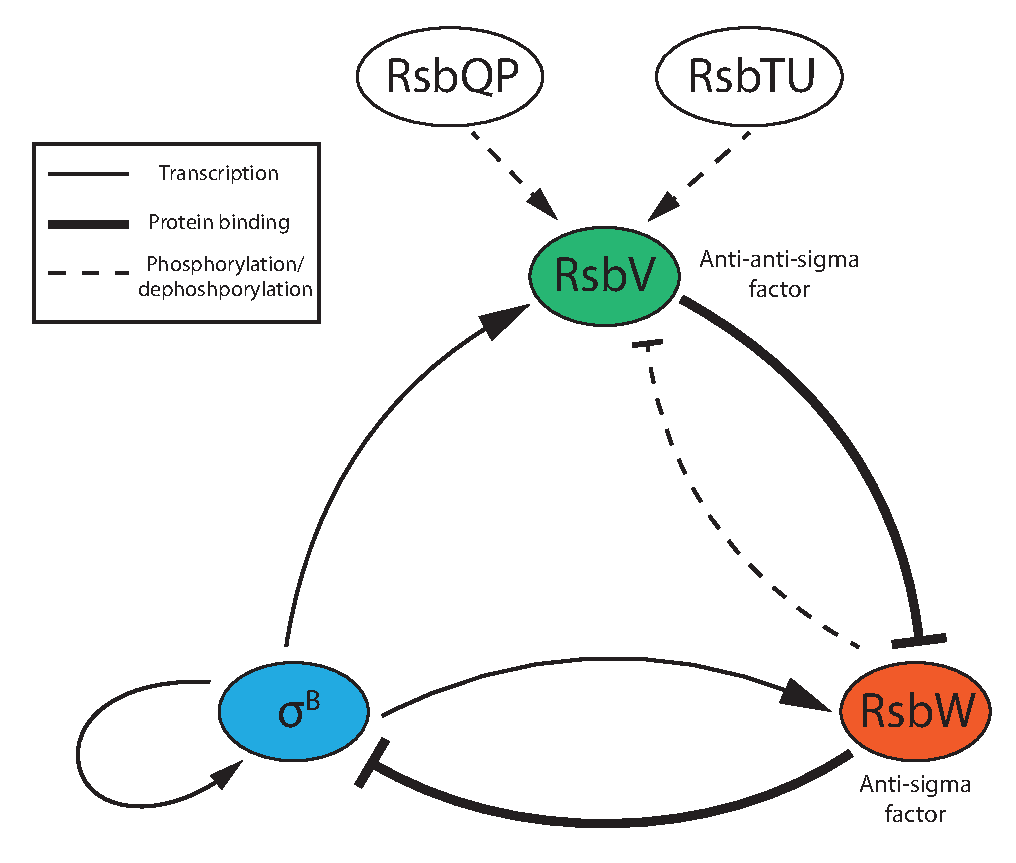
\includegraphics[width=4in]{sigB_circuit.pdf}
    \caption[
        A schematic for $\sigma^B$ gene regulation circuit.
        ]{
        \textbf{A schematic for $\sigma^B$ gene regulation circuit.}
        Type of gene/protein interaction are represented by
        different line styles.
        Pointed-end arrow denotes activation and blunt-end
        arrow denotes repression.
    }
    \label{fig:sigB_circuit}
\end{figure}

\subsection{Shared core circuit structure}
\label{sec:shared_circuit_structure}

The sigma-anti-sigma factor circuit may represent a general
regulatory mechanism for bacteria sigma factors.
Besides the aforementioned existence of $\sigma^B$ circuit
in the gram-positive relative species,
the sporulation-related sigma factors $\sigma^F$, $\sigma^E$,
and $\sigma^G$ in \textit{B. subtilis} can also be
inhibited by corresponding anti-sigma factors \cite{martinez-lumbreras18}.
Noticeably, the anti-sigma factor of $\sigma^F$, SpoIIAB,
is a kinase and can phosphorylate the anti-anti-sigma factor,
SpoIIAA. SpoIIAA can only associate with SpoIIAB when
dephosphorylated, which simulates the RsbV-RsbW-$\sigma^B$
circuit \cite{haldenwang95}.
The same structure reoccurs in \textit{E. coli}, e.g.,
the proteolysis of the general stress response sigma factor
RpoS (alias $\sigma^S$ or $\sigma^{38}$) depends on
a regulator, RssB, which serves as an anti-sigma factor
and is located in a RpoS-induced regulon.
In summary, the negative feedback loop of sigma factor conferred
by anti-sigma factor could be a general regulatory mechanism
across different bacteria species and different sigma factors
\cite{trevino-quintanilla13}.
This shared structure is reflected in the mathematical 
model for later analysis (Section~\ref{sec:low_CN}).

\subsection{Sigma factor competition}
\label{sec:intro_sigma_competition}

Besides the strict negative regulation shared among
alternative sigma factors, shifting away from the
housekeeping transcription pattern is also protected
against by the competition between sigma factors
for limited RNAP core enzymes.
%%
Sigma factor competition has been establish based on
the observation that altering housekeeping sigma factor
concentration affects the strength of alternative
sigma factor-induced stress response,
through overexpression/suppression of the housekeeping
sigma factor \cite{hicks96} or modifying the binding affinity of 
the alternative sigma factor to RNAP core \cite{zhou92a}.
%%
The alternative sigma factors (e.g. $\sigma^B$ of \textit{B. subtilis})
are at a disadvantage in the competition against the housekeeping
one since
(\textit{a}) The alternative sigma factors have weaker binding affinity
to RNAP cores than the housekeeping one, ranging from
1.5- to around 10-fold weaker \cite{maeda00,ganguly12}.
(\textit{b}) The amount of housekeeping sigma factors exceeds
significantly that of the alternative ones, even under stress
\cite{osterberg11,jishage95}.
%%
Also, considering that RNAP core and housekeeping sigma factor
roughly remains a constant level in different cell states \cite{osterberg11},
the pool of available RNAP cores for the alternative sigma factors
is capped and the competition between them can be fierce,
which is reflected a competition model that 
I developed during my research
(Section~\ref{sec:sigma_competition_model}).

\section{Biochemical ultrasensitivity}
\label{sec:biochemical_ultrasensitivity}

In the context of gene regulation, ultrasensitivity describes a sigmoidal,
switch-like increase or decrease of the expression of a gene along
increasing concentration of the regulator \cite{ferrell14a}.
%%
Namely, the dose-response curve of gene expression against regulator
concentration features a threshold, where the change of expression rate
is maximized (or "ultrasensitive" in the vicinity).
%%
The most common molecular mechanism of ultrasensitivity is binding
cooperativity, where multiple copies of the regulators associate and
together plays a role in the regulation (e.g. binds to the promoter
to initiate transcription).
%%
Conventionally, the strength of activation/repression of gene expression
is captured by the mathematical formalization of the Hill equation
\cite{hill13,alon06},
%%
where the exponent is referred to as the Hill coefficient ($n$).
When $n = 1$, the Hill equation is also referred to as the Michaelis-
Menten equation \cite{michaelis13,john12}.
%%
In equilibrium, Hill coefficient represents the number of
regulator monomers that agglomerate to form an multimer \cite{alon06}.
%%
However, often due to the lumped nature of gene expression models
(e.g. combined transcription and translation steps) and sources of
ultrasensitivity other than binding cooperativity (e.g.
multi-site phosphorylation and molecular sequestration \cite{ferrell14b}),
the Hill coefficient is an apparent parameter and is appropriate
for quantification of ultrasensitivity in the system \cite{ferrell14a}.
%%
Ultrasensitivity is crucial for a wide range of biochemical processes,
e.g., signal transduction and the maintenance of oscillation and 
bistability \cite{ferrell14c,gardner00c}.
%%
In the context of sigma factor dynamics, ultrasensitivity is needed
to explain the heterogeneity of the activation of $\sigma^V$,
where bistability is implied \cite{schwall21a}.
%%
However, there is no known binding cooperativity in most sigma
factor regulatory circuits, with one of the exceptions of \textit{B. subtilis}
$\sigma^B$ circuit, where the anti-sigma factor RsbW dimerizes and 
bind to either $\sigma^B$ or RsbV \cite{dufour94}.
The RsbW homodimer can either associate one or two monomers of
RsbV \cite{narula16}.
%%
Contradictions between the stochastic state-switching in sigma factor
dynamics and the lack of established source of ultrasensitivity
is one the main themes that I attempt to address in this thesis.

%!TEX root = ../thesis.tex
%*******************************************************************************
%****************************** Second Chapter *********************************
%*******************************************************************************

\chapter{Methods}

\ifpdf
    \graphicspath{{Chapter2/Figs/Raster/}{Chapter2/Figs/PDF/}{Chapter2/Figs/}{Figs}}
\else
    \graphicspath{{Chapter2/Figs/Vector/}{Chapter2/Figs/}{Figs}}
\fi

\section{A general model for the dynamics of alternative
 sigma factors}
% originally the equations are listed under a subsection
% related to low copy numbers. Now it is moved under the
% main title, but the tag is retained.
\label{sec:low_CN}

To further investigate the relationship between sigma factor dynamics
and the circuit 
% here I was trying to link to phenotypic variations, but seems weird
structure, i.e. how the molecules in a sigma factor network interact
with each other,
I formalized a simplified but mechanistic model to describe the system.
The model is then simulated using the Gillespie algorithm to ensure
accuracy under low copy number of molecules.
The various dynamical behaviours produced by the model may not only
serve as a theoretical explanation of the observed dynamics,
but also may give insights into other potential behaviours
(e.g. Figure~\ref{fig:different_behaviours}).
From there, I further discussed how bistability may arise without
binding cooperativity in the circuit,
a phenomenon that was not clearly accounted for in previous studies.
To accommodate the Gillespie algorithm, the system is described 
as master equations
(adopted from Torkel Loman's unpublished work):

\begin{equation}    % to give only one label to equations
\label{eqn:master_eqn}
\begin{gathered}    % for some reason, gather does not work here...
    \sigma\quad\xrightarrow{\quad \frac{\beta}{\tau_S}\left(
        v_0 + v_H\right)\quad}\quad\sigma + 1\\
    \sigma\quad\xrightarrow{\quad \frac{1}{\tau_S}\sigma \quad}
        \quad\sigma - 1\\
    A\quad\xrightarrow{\quad \frac{\beta}{\tau_A}\left(
        v_0 + v_H\right)\quad}\quad A + 1\\
    A\quad\xrightarrow{\quad \frac{1}{\tau_A}A \quad}\quad A - 1
\end{gathered}
\end{equation}

The state of the system is determined by two variables:
the copy number of the sigma factors ($\sigma$) and the copy number
of anti-sigma factors ($A$).
The probability of the transition between adjacent states
(i.e. the production or degradation of a single sigma factor/anti-sigma
factor) is a function of the current $\sigma$ and $A$.
The corresponding transition probabilities are shown above the
arrows, where $v_0$ is the basal expression rate (a constant)
and $v_H(\sigma, A)$ is the primary expression rate.
Here, $v_H(\sigma, A)$ is derived from binding kinetics and
reflects the circuit structure.
Other parameters include $\beta$, the maximum expression rate,
and $\tau_S$ and $\tau_A$, which are respectively the (average)
molecular lifetime of $\sigma$ and $A$.
The primary expression rate $v_H$ is written as:

\begin{align}
    v_H = \frac{\sigma/K_S}{\sigma/K_S + (A/K_D)^n + 1}
\end{align}

Where $K_S$ and $K_D$ are two different dissociation constants which
reflect the binding equilibriums of the system.
$n$ here is the apparent binding cooperativity, which is an indicator
of ultrasensitivity.
However, as mentioned previously in Section~
\ref{sec:biochemical_ultrasensitivity}, many sigma factor circuits
do not have known binding cooperativity, but whose observed
dynamical behaviours are suggested to rely on ultrasensitivity.
I will revisit this parameter $n$ later.

Though may be obscured by the formalization required by the 
Gillespie algorithm, the model (Eq.~\ref{eqn:master_eqn}) generally
depends on only two major assumptions, namely

\begin{itemize}
    \item The circuit only contains two protein species: the sigma
    factor ($\sigma$) and the anti-sigma factor ($A$).
    \item The sigma factor is under positive autoregulation, but
    also under negative feedback through the anti-sigma factor.
\end{itemize}

Besides the well-studied $\sigma^B$ factor, other sigma factors
such as $\sigma^D$, $\sigma^W$, and $\sigma^X$ 
\cite{haldenwang95, huang98, hsueh11} can all be 
abstracted in a such way in line with these assumptions.
Other assumptions include that the binding events are much
faster than transcriptions so that binding is considered to be
at equilibrium, and, similarly, that translation is much 
faster than translation, so that the expression rate is the
combination of the two, etc.


%%%%%%%%%%%%%%%%%%%%%%%%
% Old writings
%%%%%%%%%%%%%%%%%%%%%%%%
% Here I propose a general model to explain the spectrum of 
% dynamical behaviours, e.g. stochastic pulsing \cite{locke11,cabeen17},
% transient pulsing and sustained activation \cite{cabeen17}
% of the bacterial alternative sigma factors in the species 
% \textit{B. subtilis}.
% It also serves as the foundation of the sigma factor competition
% model (Section~\ref{sec:sigma_competition_model}).
% The model is based on the general topology that is 
% shared by multiple alternative sigma factor networks
% including $\sigma^D$, $\sigma^W$, $\sigma^X$, etc
% \cite{haldenwang95, huang98, hsueh11}, namely

% \begin{itemize}
%     \item The sigma factor is under positive autoregulation, i.e.,
% the sigma factor activates its own expression.
%     \item An anti-sigma factor is co-expressed with the sigma factor as its
% inhibitor, forming a negative feedback loop.
% \end{itemize}

% I formalize a minimal mechanistic model based on these network topologies.
% Without loss of generality, the following model reflects the $\sigma^B$
% regulatory network but is applicable to other alternative sigma factors.

\subsection{Sigma-anti-sigma binding kinetics}

The primary expression rate, $v_H$, which is expressed as a Hill function
(thus the denotation), is derived from the binding kinetics between the
sigma factor and the anti-sigma factor,
and that between the RNAP holoenzyme (comprising the sigma factor) and the promoter.
Notice that $v_H$ is shared by the production step of both the sigma factor
and the anti-sigma factor, since they are located in the same operon.
%%
First, the promoter of the operon including the gene that encodes the sigma factor
is transcribed by the RNA polymerase (RNAP) holoenzyme comprising 
the sigma factor itself.
The relative transcription rate (denoted by $v_H$) to the maximal rate 
is modelled by Hill kinetics with ultrasensitivity encoded in $n$:

\begin{align}
    \label{eqn:v_hill}
    v_H = \frac{\sigma_f^n}{K_S^n + \sigma_f^n}
\end{align}

where $\sigma_f$ is the abundance of the unbound sigma factors, as
the anti-sigma factor (denoted by $A$), competes the binding of 
sigma factors with RNAP cores.
$K_S$ is the dissociation constant between the RNAP holoenzyme and the promoter.
$n$ is the Hill coefficient, which represents the apparent binding cooperativity.

Second, the anti-sigma factor ($A$) sequesters the sigma factor ($\sigma$)
from the RNAP core by binding to it and forming a complex (denoted by $A\sigma$).
As the binding is on a faster time scale than transcription,
the binding dynamics can be considered at steady-state in
transcriptional regulation.
The binding dynamics is governed by 

\begin{gather}
    \label{eqn:W_binding}
    K_D = \frac{A_f\cdot \sigma_f}{A\sigma}\\
    \label{eqn:total_sigma}
    \sigma = \sigma_f + A\sigma
\end{gather}

where $\sigma$ is the total abundance of sigma factors
and $A_f$ is the amount of unbound anti-sigma factors.
$K_D$ is the dissociation constant of sigma-anti-sigma factor binding.
Together, Eq.~\ref{eqn:W_binding} and Eq.~\ref{eqn:total_sigma}
bridges the abundance of free sigma factors and 
the total number of sigma factors as

\begin{align}
    \label{eqn:sigma_f}
    \sigma_f = \frac{K_D}{K_D + A_f}\sigma
\end{align}

i.e. the binding is subject to Michaelis-Menten kinetics,
which, in the general model described here, is considered
as non-cooperative.
Finally, under the assumption that the anti-sigma factor is in excess
to the sigma factor so that $A \approx A_f$,
Eq.~\ref{eqn:v_hill} can be re-written as

\begin{align}
    \label{eqn:v_hill_2}
    v_H = \frac{(\sigma/K_S)^n}{(\sigma/K_S)^n + (A/K_D + 1)^n}
\end{align}

Given Eq.~\ref{eqn:v_hill_2} where ultrasensitivity is derived from
the cooperativity of transcription initiation,
there are other steps in the core sigma factor network that can
potentially contribute to $n$,
e.g., for $\sigma^B$ network, RsbW dimerizes to bind $\sigma^B$, which
is captured by as $\sigma_f = K_D^2/(K_D^2 + A_f^2)\cdot\sigma$.
Generalization leads to an alternative form of Eq.~\ref{eqn:v_hill_2}
where the cooperative binding between sigma factors and anti-sigma factors
solely accounts for the ultrasensitivity.

\begin{align}
    v_H = \frac{\sigma/K_S}{\sigma/K_S + (A/K_D)^n + 1}
\end{align}

\subsection{Activation of the circuit}

Here I take the $\sigma^B$ circuit as an example to explain the model.
Upon exposure to the stressor,
a phosphatase, either RsbQP or RsbTU is released, depending on whether the
environmental stress or energy stress is applied.
This process in turn dephosphorylates the anti-anti-sigma factor RsbV to
its activated form (which the activated from is denoted by $V$).
RsbV competes the binding of RsbW with $\sigma^B$, which releases
$\sigma^B$ and, thus, triggers the stress response.

Similar to Eq.~\ref{eqn:sigma_f}, at steady-state,
the abundance of RsbW free to RsbV binding is captured 
by Michaelis-Menten kinetics

\begin{align}
    \label{eqn:A_f}
    A_f = \frac{K_A}{K_A + V}A
\end{align}

Notice that the $A$ term in Eq.~\ref{eqn:v_hill_2} is essentially the unbound
anti-sigma factor, which, according to Eq.~\ref{eqn:A_f},
is a function of the activated RsbV and 
the total amount of anti-sigma factors.
Substituting Eq.~\ref{eqn:A_f} in to Eq.~\ref{eqn:v_hill_2}, we then have

\begin{align}
    v_H = \frac{(\sigma/K_S)^n}
        {(\sigma/K_S)^n + \left(\frac{A}{(1 + V/K_A)K_D} + 1\right)^n}
\end{align}

Here, I define the apparent sigma-anti-sigma dissociation constant as
$K_D' = (1 + V/K_A)\cdot K_D$, which then keeps the mathematical form
of Eq.~\ref{eqn:v_hill_2} unchanged.
Thus, upon stress, the step-increase in the
abundance of dephosphorylated RsbV is modelled by a step-increase
of the apparent $K_D$.

Admittedly, not every sigma factor circuit includes an anti-anti-sigma factor,
thus the derivations above are not readily applicable to other 
sigma factor circuits.
However, for simplicity, it is still reasonable to model the activation
of the system as a step-change in the parameter $K_D$,
as it may also represent the effect of activation
ignorant of the actual mechanism.



\subsection{Modelling stochastic fluctuation under low copy number}

The alternative σ factors typically exist in low copy number and,
thus, their abundance is subject to stochastic fluctuation.
In \textit{Escherichia coli}, while there can be thousands of housekeeping
$\sigma^{70}$ factor per cell, the number of alternative $\sigma^E$
factor is only about 160 even under stress \cite{collinet00}.


Since noise can be crucial to the pulsing dynamics \cite{park18a},
and that noise is stronger under low copy numbers,
I model the system with the Gillespie algorithm to ensure the 
accuracy of simulation when the molecular abundance is low.
The model expressed in master equations is shown in
Eq~\ref{eqn:master_eqn}.

% I model the system with the exact molecular number of
% the alternative σ factor ($\sigma$) and the anti-sigma factor
% ($A$) as the state variables,
% and the random walk through state-space with jump events
% (based on the unpublished work of Torkel Loman):

% \begin{gather}
%     \sigma\quad\xrightarrow{\quad \frac{\beta}{\tau_S}\left(
%         v_0 + v_H\right)\quad}\quad\sigma + 1\\
%     \sigma\quad\xrightarrow{\quad \frac{1}{\tau_S}\sigma \quad}
%         \quad\sigma - 1\\
%     A\quad\xrightarrow{\quad \frac{\beta}{\tau_A}\left(
%         v_0 + v_H\right)\quad}\quad A + 1\\
%     A\quad\xrightarrow{\quad \frac{1}{\tau_A}A \quad}\quad A - 1
% \end{gather}

% where the relative transcription rate, $v_H$ is given
% by Eq.~\ref{eqn:v_hill_2}.
% The transcription rate is generalized which also 
% accounts for translation.
% $v_0$ is the basal transcription activity and $\beta$ is the maximal
% transcription rate, which determines the steady-state abundance.
% If steady-state is reached, the average abundance of both species
% equals to $\beta v_H$ (ignoring basal transcription),
% i.e. $\langle \sigma \rangle = \langle A \rangle$.
% The same primary transcription rate is shared between $\sigma$ and $A$
% since they are co-expressed in the same operon.

The parameters used in the model or its derivation are summarized
in Table~\ref{tab:general_model_paras}.

\begin{table}[ht]
    \centering
    \begin{tabular}{|c|p{3.5in}|c|}\hline
        Parameter & Description & Units\\\hline
        $K_S$ & Dissociation constant between the sigma factor-
        RNAP core complex and the promoter & Molecules per cell\\
        $K_D$ & Dissociation constant between the sigma factor
        and the anti-sigma factor & Molecules per cell\\
        $K_A$ & Dissociation constant between the anti-sigma factor
        and the anti-anti-sigma factor & Molecules per cell\\
        $\tau_S$ & Average molecular lifetime of the sigma factor &
        Arbitrary units\\
        $\tau_A$ & Average molecular lifetime of the anti-sigma factor &
        Arbitrary units\\
        $\beta$ & Maximal expression rate of the operon containing the sigma
        factor and the anti-sigma factor when fully activated
        & Molecules per cell\\
        $v_0$ & Scaled basal expression rate of the operon & -\\
        $v_H$ & Scaled primary expression rate of the operon & -\\\hline
    \end{tabular}
    \caption[Parameter list of the sigma factor model]
    {\textbf{Parameter list of the sigma factor model}}
    \label{tab:general_model_paras}
\end{table}

\subsection{Nondimensionalization of time}
\label{sec:methods_nondim_time}    % there is a similar section in discussion

Though the chemical species are measured in absolute number of molecules (per cell),
the quantities related with time, such as molecular lifetime and
the reaction rates, are on a relative scale.
The Gillespie algorithm is not dependent on the time scale that one chooses,
which warrants this nondimensionalization of time.
Also to support it, I measured the variation of the copy number of sigma factors
at equilibrium when the system is in the dynamical regime of 
constant expression.
The variation remains the same when changing the absolute unit of time
(but keeping the relative amounts).
To be specific, the average lifetime of the sigma factor is set to 10
units of time for most simulations, while the lifetime of the anti-sigma
factor is 50, being 5 times longer than that of the sigma factor.
This settings ensures a delay in the negative feedback (through the 
anti-sigma factor) relative to the self-activation of the sigma factor.
I suggest that the delay is essential for some behaviours, e.g.,
oscillation. Specifically, oscillation cannot maintain if the lifetime of 
the anti-sigma factor is smaller than that of the sigma factor, i.e.,
if without delay in the negative feedback loop (data not shown).
Though the idea is not fully developed in this thesis,
it may be as interesting a topic as exploring the influence of ultrasensitivity
to ask what is the role of delay in the circuit.


\section{Simulation of the model}

The model is simulated by the Gillespie algorithm, i.e. the
Stochastic Simulation Algorithm \cite{gillespie77},
which generates statistically accurate trajectories of the
jump processes described in Section~\ref{sec:low_CN} as
a Markov process.
The algorithm I used is provided by the Catalyst.jl \cite{catalystjl} package,
which an interface around DifferentialEquations.jl \cite{rackauckas17},
of the Julia language \cite{Julia-2017}.


\section{A sigma factor competition model}
\label{sec:sigma_competition_model}

% "dual" sigma factor model
To explore the emerged dynamics from the competition of different
sigma factors for limited RNAP core enzymes,
I built a model consisting of two sigma factor circuits,
whose biochemical parameters ($n$, $K_S$, $K_D$, etc.) are independent.
%%
For simplicity, the model only focuses on two of the various 
alternative sigma factors (for context, \textit{B. subtilis} has 17 
different alternative sigma factors \cite{park18a}).
%% 
% the actual number of RNAP cores is addressed in either 
% parameters or discussion
The influence of the remaining sigma factors, including the 
housekeeping one, is averaged and reflected by the limited
number of available RNAP cores.
%%
In addition to the model of the core circuit (Section~\ref{sec:low_CN}),
the competition model links the two sigma factors by 
the association to and dissociation from a shared pool of
RNAP cores:

\begin{gather}
    E + \sigma \quad \xrightarrow{\quad k_{on} \quad} \quad E\sigma\\
    E\sigma \quad \xrightarrow{\quad k_{off} \quad} E + \sigma
\end{gather}

Where $E$ is the RNAP core enzyme and $\sigma$ represents
either of the two competing sigma factors.
%%
The reaction rate follows the law of mass reaction (considering
elementary reactions) with the association rate constant $k_{on}$ and
dissociation rate constant $k_{off}$.
%%
The rate constants relate to the equilibrium binding affinity 
(expressed by the dissociation constant $K_{E\sigma}$) by
\cite{john12}

\begin{align}
    \label{eqn:disso_constant_to_rates}
    K_{E\sigma} = \frac{k_{off}}{k_{on}}
\end{align}

The total amount of RNAP cores, captured by $E + E\sigma$
in the model, is essentially the pool of RNAP cores that
are accessible to the two sigma factors here subtracting
the proportion already bound by the housekeeping sigma factor and
other alternative ones.
%%
This value is assumed constant since both the total 
RNAP cores (shared by all sigma factors) and the housekeeping
sigma factors remain relatively constant in different
growth conditions \cite{osterberg11}.
%%
Admittedly, the assumption is impaired by the fluctuating 
amount of other alternative sigma factors, 
which motivates a multi-sigma factor competition model in
future study.


% I put this after the competition model to allow a further 
% explanation of those parameters
\section{Model parameters}

% why we care about the actual values of the parameters
The values of the parameters matter since the behaviour of the system
can change drastically when tuning some of the parameters,
e.g. when changing $n$ that represents ultrasensitivity.
The parameters are of biological significance.
Thus, the validity of the model partially depends on whether
the parameters match actual measurements.
% the general model
For most simulations, $\beta$ is set to 50.
This parameter dictates the equilibrium number of sigma factors
per cell when the expression of sigma factor is activated,
which aligns with the literature value from tens to thousands
\cite{collinet00,mauri14} but is on the fewer side to emphasize
the effects of fluctuations at low copy number.
As mentioned in Section~\ref{sec:methods_nondim_time},
the units of time is arbitrary, but to allow some dynamical behaviours,
e.g. oscillation, the average lifetime of the sigma factor should
be shorter than that of the anti-sigma factor ($\tau_S < \tau_A$).

% now the competition model
In the sigma factor competition model, the dissociation constant
between the sigma factor and the RNAP core ($K_{E\sigma}$) contributes crucially
to the strength of the competition.
A study reports that the constant can range from ~1 to more than 100
molecules per cell (in typical bacteria, \SI{1}{\nano\Molar} converts
to approximately 0.8 molecules per cell),
which sets the range of the simulation in this thesis.
RNAP holoenzyme forming kinetics, characterized by the rates
$k_{on}$ and $k_{off}$ are also ruled by $K_{E\sigma}$ through
Eq~\ref{eqn:disso_constant_to_rates} (more discussed in
Section~\ref{sec:discussion_parameters}).
Finally, it is important to point out that given the degree of
simplicity and some presumptions used in the model,
more accurate measurements of the biological system does not
necessarily improve the predictability of the model.
The model is meant to provide insights on how the circuit is 
tuned by several biophysical properties of the molecules.
Thus, it is still important to assess the system under
certain changes and then evaluate the predictions given by this model.


% Notes: the algorithm lies at the core of the thesis
% but is painful to formally write it down.
% partially because it evolves over time and, awkwardly,
% it relies on several hard-coded, even fine-tuned parameters
\section{A classification algorithm for dynamical behaviours}
\label{sec:classification_algorithm}

% goal of the algorithm
To effectively explore how the different behaviours generated by the model
with different parameters,
I developed the automatic classifier.
The classification algorithm described here takes the 
discrete-valued trajectories of a two-species reaction system as
the input and classifies the system as one of
the qualitatively distinct behaviours.
% an overall description of the algorithm
The pre-stress (i.e. pre-perturbation) trajectory is truncated before further analysis.
The classification is done by examining the phase-plane 
(i.e., the $\sigma$-$A$ plane) characteristics.
Since the system written in discrete master equations (Eq. \ref{eqn:master_eqn})
instead of ODEs, I will first reconstruct the flow by estimating
the vector field from the Gillespie-simulated trajectories as described in
Section \ref{sec:reconstruction}.

Inspired by continuous models, I located the "fixed points" of the system
which are the maxima of the density of the trajectories.
Combined with the"flow" across the fluctuation threshold (detailed in Section \ref{sec:detecting_fp}), etc.
and Fourier analysis of the trajectory,
the algorithm determines the type of dynamics by a decision tree
(Figure~\ref{fig:classifier_flowchart}).

\subsection{Reconstructing the vector field from simulation}
\label{sec:reconstruction}

In my algorithm, the reconstructed vector field and the trajectory densities
are important for identifying the fixed points, and thus,
for determining the behaviour types.
%
First, the trajectory density, $I$, is defined at each lattice point 
$(\sigma, A)$ as the number of times that the post-stress trajectory passes
that point.
%
Then, the vector field requires the gradient at each lattice point.
The gradient at point $(\sigma_k, A_k)$ is denoted as 
$(\dot{\sigma}_k, \dot{A}_K)$. It is calculated in a manner similar to
the symmetric derivative at $(\sigma_k, A_k)$ and is averaged
among all the times that the trajectory passes $(\sigma_k, A_k)$.
Formally, the two components of the gradient are

\begin{align}
    \dot{\sigma}_k &= \frac{1}{I(\sigma_k, A_k)}\sum_{t \in T_k}
    \frac{\sigma(t + \Delta t) - \sigma(t - \Delta t)}{2\Delta t}\\
    \dot{A}_k &= \frac{1}{I(\sigma_k, A_k)}\sum_{t \in T_k}
    \frac{A(t + \Delta t) - A(t - \Delta t)}{2\Delta t} \text{,}
\end{align}

where $I(\sigma_k, A_k)$ is the trajectory density at point $(\sigma_k, A_k)$,
$T_k$ is the set of time points where the trajectory passes
$(\sigma_k, A_k)$, 
formally $T_k = \left\{t|\sigma(t) = \sigma_k \;\text{and}\; A(t) = A_k\right\}$,
and $\Delta t$ is the time step of the simulation.

% First, the algorithm recreates the phase-plane paths and the 
% vector field of time-derivatives from the trajectories.
% The intensity ($I$) of phase-plane path of each lattice point on the 
% phase plane is calculated as the total number of times that
% the path passes the point.
% The time-derivative at the point $(\sigma_k, A_k)$ is approximated by

% \begin{align}
%     \dot{\sigma} &= \frac{1}{I(\sigma_k, A_k)}\sum_{t_k}
%     \frac{\sigma(t_k + \Delta t) - \sigma(t_k - \Delta t)}{2\Delta t}\\
%     \dot{A} &= \frac{1}{I(\sigma_k, A_k)}\sum_{t_k}
%     \frac{A(t_k + \Delta t)- A(t_k - \Delta t)}{2\Delta t}
% \end{align}

% where $t_k$ are the time points after exposure to stress which satisfies
% $\sigma(t_k) = \sigma_k \text{and} A(t_k) = A_k$.
% More explicitly, the phase-plane path travels to $(\sigma_k, A_k)$ at time $t_k$.

\subsection{Detection of fixed points and "flows" across the fluctuation thresholds}
\label{sec:detecting_fp}
%
For continuous models e.g. ODEs, if a stable fixed point exists,
trajectories in the \emph{basin of attraction} of the fixed point will eventually
converge to it.
This results in a high trajectory density about the stable fixed point.
The maxima of the density of a Gillespie trajectory plays a similarly important
role to announce the type of dynamics of a discrete model.
For the sake of argument, I will call these maxima as the "fixed points" of
the discrete model.
Notice that the maxima of density do not necessarily behaviour in the way
of stable fixed points of ODEs.
E.g., The Gillespie trajectory in Figure \ref{fig:density_and_vf} behaviours as a homoclinic
connection, a circle solution connecting to a saddle.
Such dynamics allow the phase point to linger around the saddle for a good amount
of time while occasionally visiting the loop, which leads to a maximum at the saddle
(Figure \ref{fig:density_and_vf} B).
We categorize this behaviour as stochastic pulsing, intuitively similar to the firing
of a neuron (see \cite{hesse22} for a model of action potential with homoclinic connections).
%
The classification algorithm relies on identifying the fixed points of the
Gillespie model. Density on the phase plane is defined as the number of times that
the trajectories visit each grid point. The densities are smoothed and
the fixed points are found at the local maxima.

The flow on the phase plane, expressed as a vector field,
is also approximated from the trajectories generated
from the stochastic model. We pay specific attention to the flow on the fluctuation thresholds

\begin{align}
    \sqrt{\sigma_x^2} = \sqrt{\beta/n}
    \label{eqn:fluc_threshold}
\end{align}

Which derives from the fluctuation-dissipation theorem\cite{paulsson05a}

\begin{align}
    \frac{\sigma_x^2}{<x>^2} = \frac{1}{n<x>}
\end{align}

Where $\sigma_x^2$ is the variance of the expression of gene $x$, namely
$\sigma_x^2 = <x^2> - <x>^2$. $n$ is the Hill coefficient.
The mean expression level at steady state $<x>$ is determined by the parameter $\beta$,
which then gives Eqn. \ref{eqn:fluc_threshold}.
Practically, I usually use twice of the theoretical threshold to distinguish
a bona fide equilibrium from excitable dynamics.
The caveats would be that (1) the choice of the fluctuation threshold determines
the type of dynamics on the boundary of two categories, e.g., a dynamics where
the flow settles most of the time but excites only rarely
and (2) the fluctuation-dissipation may not be applicable for out-of-steady-state
systems\cite{chabot07}.
The flow crossing the $\sigma$-axis or the $A$-axis are denoted as the forward flow
$I_{forward}$ or the reverse flow $I_{reverse}$ respectively.
Both of the flows and the existence of "fixed points" are then feed into the 
algorithm to decide the type of dynamics.

\begin{figure}
    \centering
    \begin{subfigure}{0.45\textwidth}
        \centering
        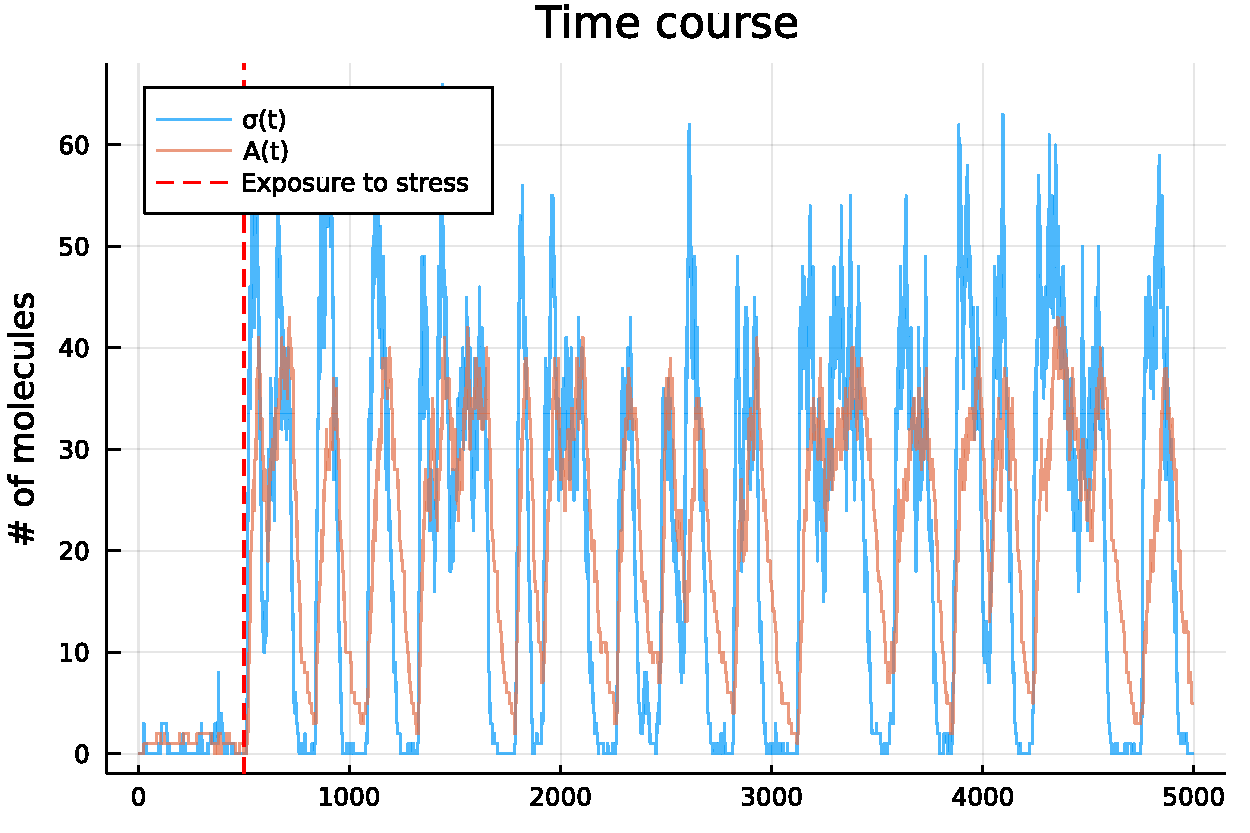
\includegraphics[width=\textwidth]{Figs/2_5_algo_example_traj.pdf}
        \caption{Trajectory}
    \end{subfigure}
    \hfill
    \begin{subfigure}{0.45\textwidth}
        \centering
        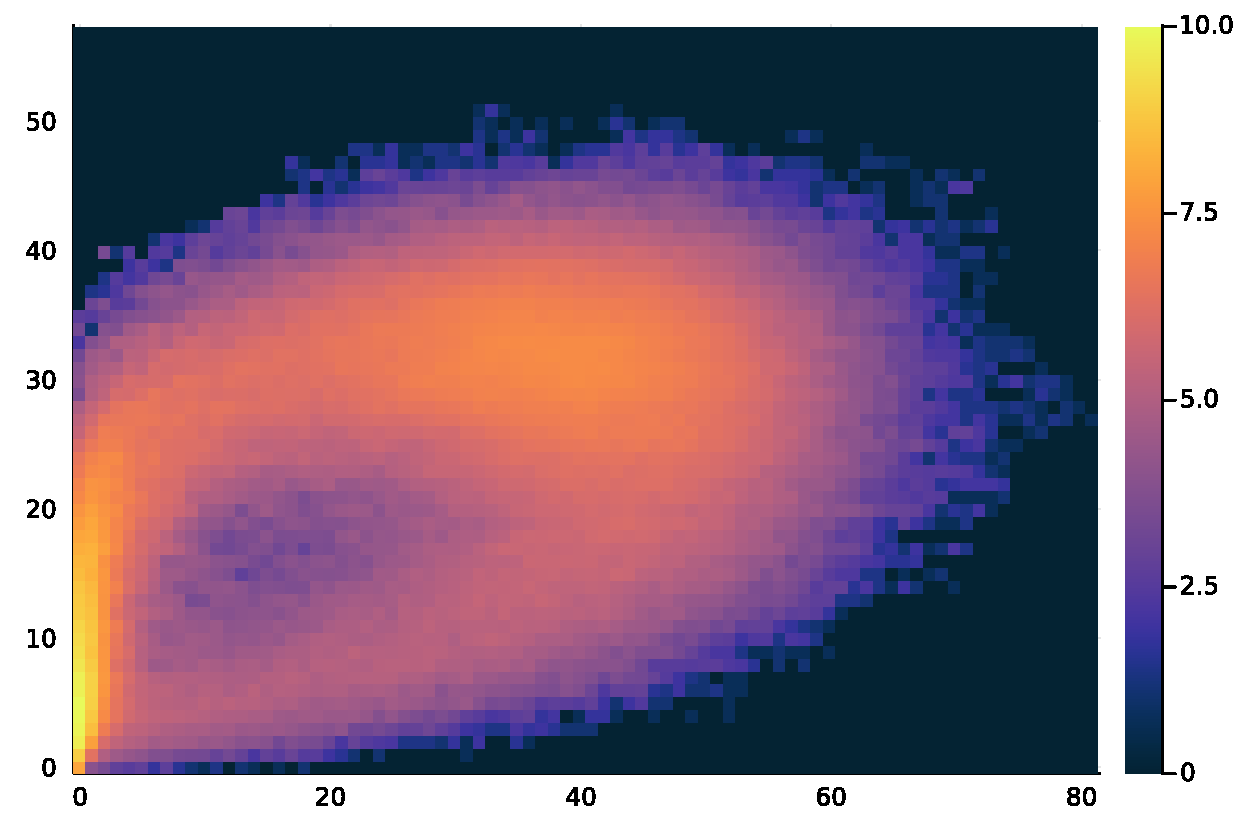
\includegraphics[width=\textwidth]{Figs/2_5_algo_example_density.pdf}
        \caption{Density}
    \end{subfigure}
    
    \begin{subfigure}{0.45\textwidth}
        \centering
        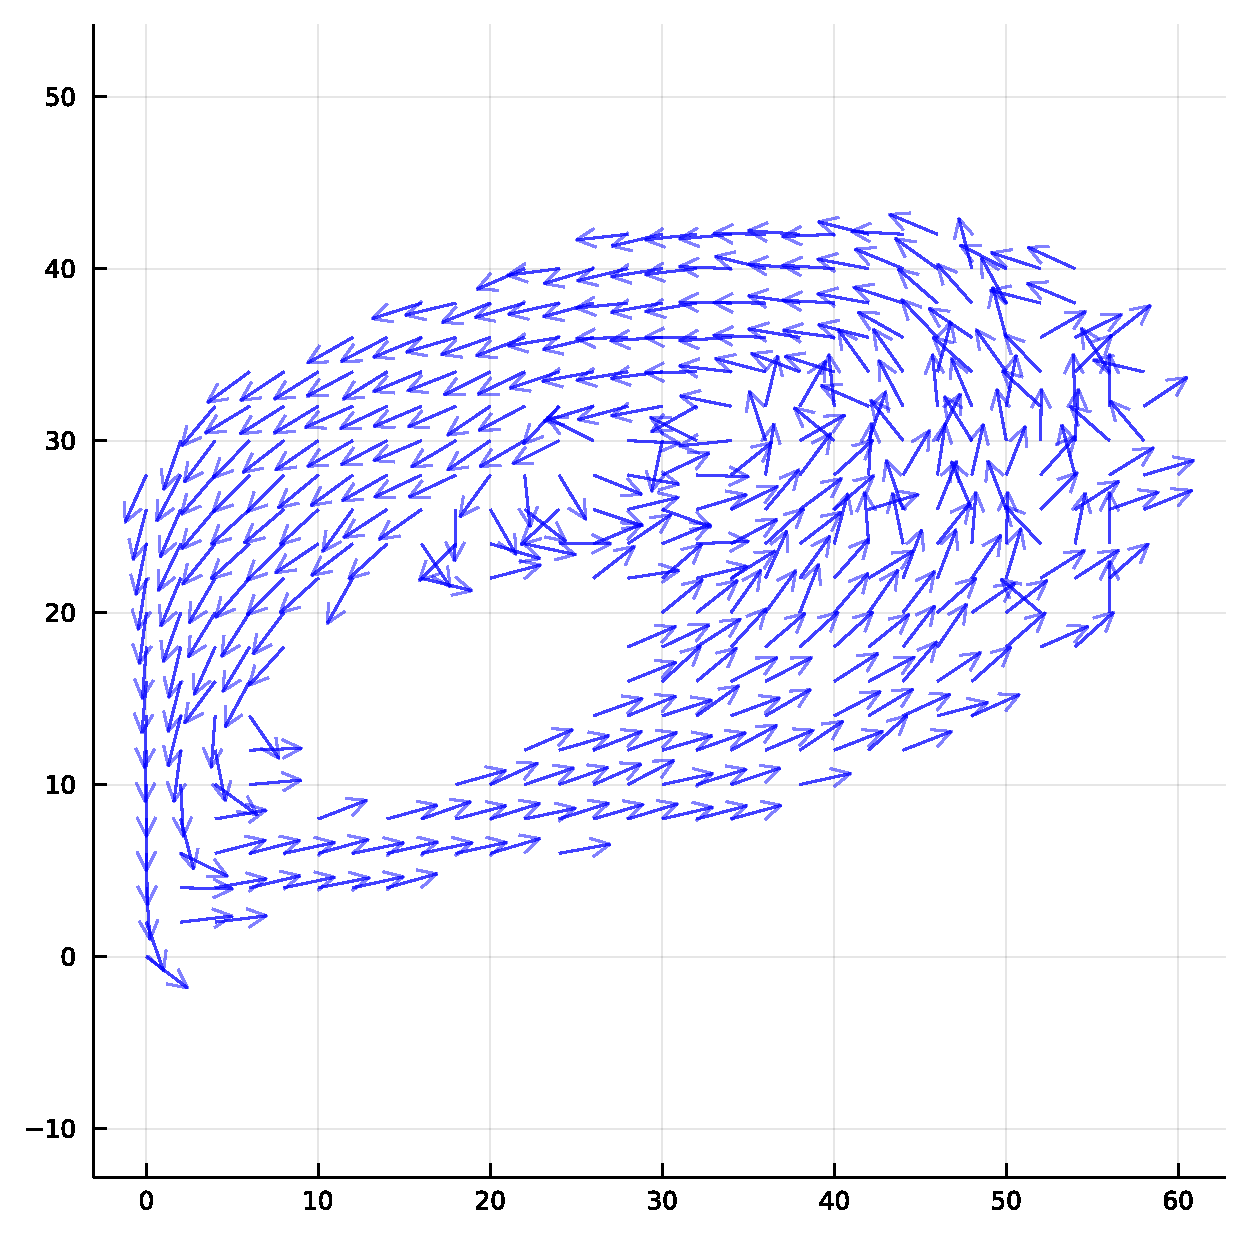
\includegraphics[width=\textwidth]{Figs/2_5_algo_example_vf.pdf}
        \caption{Vector field}
    \end{subfigure}
    \caption[Example trajectory of the discrete model, density on the phase plane,
    and reconstructed vector field]
    {Example trajectory of the discrete model, density on the phase plane,
    and reconstructed vector field}
    \label{fig:density_and_vf}
\end{figure}

Finally, Figure~\ref{fig:classifier_flowchart} shows the flowchart
to decide the classification, where
$N_{small}$ is the number of stable fixed points where the abundance
of both species are greater than the threshold $T_{fluc}$,
and similarly, $N_{large}$ is the number of stable fixed points
which the abundance of both species are less than $T_{fluc}$.
$I_{forward}$, or the forward flow, is defined as the sum of 
intensity on the vertical segment from $(T_{fluc}, 0)$ to 
$(T_{fluc}, T_{fluc})$.
Similarly, the reverse flow $I_{reverse}$ is the sum of intensity
on the horizontal segment from $(0, T_{fluc})$ to $(T_{fluc}, T_{fluc})$.



\begin{figure}[ht]
    \centering
    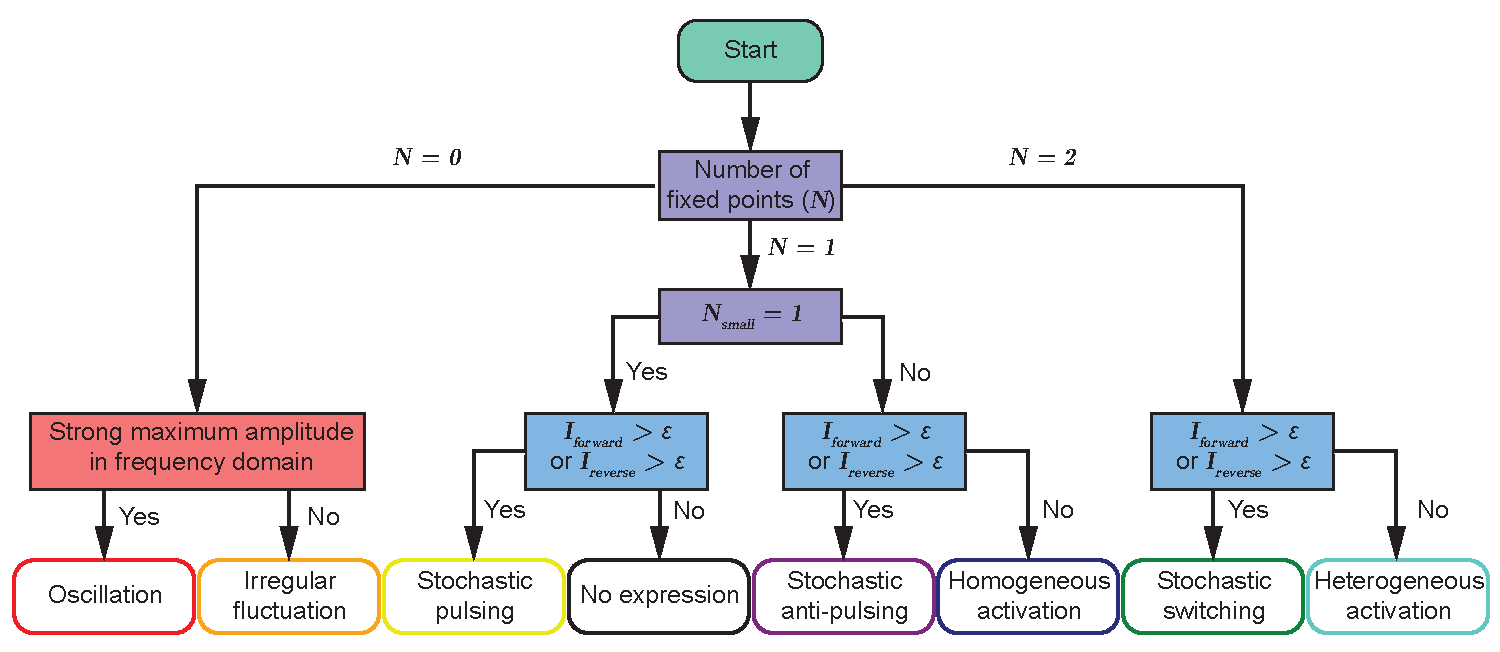
\includegraphics[width=6in]{classifier_flowchart_remake}
    \caption[The decision tree for different behaviour types] {
        \textbf{The decision tree for different behaviour types} lies at
        the core of the classification algorithm. Several phase-plane
        properties are reconstructed from the Gillespie-simulated trajectories.
        The phase-plane properties determine the behaviour types.
        $N$ is the number of fixed points. $N_{small}$ is the number of
        fixed points close to the origin, which are formally the ones below
        the fluctuation threshold.
        $I_{forward}$ and $I_{reverse}$ are respectively the forward and
        reverse flow of the trajectory across the fluctuation threshold.
        $\epsilon$ is a small amount. I used $\epsilon = 1 \times 10^{-4}$
        in the algorithm.
        A strong maximum amplitude is defined as that the maximum amplitude 
        $> 50$ folds of the average of its vicinity.
    }
    \label{fig:classifier_flowchart}
\end{figure}

% I don't have time to develop this section
% admittedly, not a very mature concept, but would be
% interesting/useful to develop it further

% \subsection{Determine the threshold from the level of stochastic fluctuation}


%!TEX root = ../thesis.tex
%*******************************************************************************
%****************************** Third Chapter **********************************
%*******************************************************************************
\chapter{Results}

% **************************** Define Graphics Path **************************
\ifpdf
    \graphicspath{{Chapter3/Figs/Raster/}{Chapter3/Figs/PDF/}{Chapter3/Figs/}{Figs}}
\else
    \graphicspath{{Chapter3/Figs/Vector/}{Chapter3/Figs/}{Figs}}
\fi

\section{Mathematical model predicts different dynamical behaviours}
\label{sec:general_diff_behaviours}
% a weird name because before I used the term "general model" to contrast
% any sigB specific model. However, later on only the "general model" is
% discussed in the thesis

% Gillespie show diverse behaviours. why Gillespie
To validate the mathematical model which is based on the biochemical processes
(Section~\ref{sec:low_CN}), I simulated the time evolution of the system 
using the Gillespie algorithm (i.e. stochastic simulation algorithm) 
\cite{gillespie77}.
Previous work shows that a similar model simulated by the chemical Langevin 
equation (CLE) exhibits diverse dynamical behaviours (unpublished work by
Torkel Loman).
% The argument that CLE is not appropriate for the simulation
% is rather long. Might want to move this to Methods
However, CLE only holds on the condition that, in a time step,
the expected occurrence of the reaction is large enough and the change
of reaction rate is small enough, both of which are facilitated by a large
number of molecules present in the system \cite{gillespie00}.
Since the simulation focuses on dynamical behaviours such as stochastic pulsing
and stochastic switching between activation and inactivation
where low-copy number is important,
these assumptions may be violated.
The Gillespie algorithm generates statistically correct trajectories
from the chemical master equations \cite{gillespie77}, 
which is important for the low-copy number
regime here and also for establishing the bistability
in Section~\ref{sec:both_non_coop_bistability} which exploits
single-molecule dynamics.

% What are the types of behaviours and where to find them
Simulated with the Gillespie algorithm,
the model (Section~\ref{sec:low_CN}) 
displays a wide range of dynamical behaviours
when changing the activating and repressive forces
(Figure~\ref{fig:different_behaviours}).
% what are activating and repressive force?
% (why I talked about K_S and K_D first? because I'll talk about
% behaviour mapping next, and the parameters link the two)
% may be don't mention threshold here?
The parameters that tune the strength of activating and repressive forces 
are $K_S$ and $K_D$, respectively.
The activating force is inversely scaled by $K_S$ and, thus,
$K_S$ is called the activation threshold (which makes sense
especially in an ultrasensitive system).
Similarly, the repressive force is inversely scaled by $K_D$,
which serves as the repression threshold
(biochemical significance see Table~\ref{tab:general_model_paras}).
% Introduce the behaviour mapping
Seven primary types of dynamical behaviours emerge from
this simulation of an ultrasensitive (Hill coefficient $n = 3$)
sigma factor circuit.
To illustrate how the strength of activating and repressive 
forces determine the type of dynamical behaviours, I mapped
the behaviours to the parametric space of $K_S$ and $K_D$,
where the different behaviours are colour-coded
(Figure~\ref{fig:different_behaviours} centre).
% A list of dynamical behaviours
The seven types of dynamical behaviours are:

\begin{enumerate}[label=(\alph*)]
    \item No expression.
    \item Stochastic pulsing, characterized by the dominance of OFF-states
    interspersed with narrow peaks of expression.
    \item Oscillation, characterized by approximately periodic switching
    between ON and OFF states.
    \item Stochastic anti-pulsing, characterized by the dominance of 
    ON-states with stochastically timed transient shutdowns.
    \item Homogeneous activation, characterized by immediate activation
    upon exposure to stress.
    \item Stochastic switching, characterized by stochastically timed
    switching between ON- and OFF-states.
    \item Heterogeneous activation, characterized by heterogeneously
    delayed activation.
\end{enumerate}

% One more behaviour
And (h) irregular fluctuation, which typically exists
in non-ultrasensitive ($n = 1$) regime.
It is an intermediate dynamical behaviour between
stochastic pulsing and activation (more discussed in
Section~\ref{sec:us_for_bs_and_oscillation}).
A short trajectory along time for each behaviour is shown
in Figure~\ref{fig:different_behaviours}.
% Areas of pulsing and activation are large
% I may inferred too far here...
The behaviour mapping in Figure~\ref{fig:different_behaviours}
shows a wide range for stochastic pulsing (yellow) and 
homogeneous activation (deep blue), suggesting that these behaviours are
robust to the biochemical parameters and thus are more likely to be
conserved through neutral selection.
% separation by K_D/K_S
% this becomes a wordy paragraph, may suits discussion
% but can (somewhat floppily) used to argue that K_D/K_S and K_S 
% independently tune the system
Certain values of the ratio $K_D/K_S$ separates dynamical behaviours
(e.g. the vertical boundary of oscillation in 
Figure~\ref{fig:different_behaviours}).
This can be understood by rewriting the Hill term from Eq.~\ref{eqn:v_hill_2}
as:

\begin{align}
    v_H =& \frac{\sigma^n}{\sigma^n + 
        \left[A/\left(\frac{K_D}{K_S}\right) + K_S\right]^n}\\
    \approx& \frac{\sigma^n}{\sigma^n + 
        \left[A/\left(\frac{K_D}{K_S}\right)\right]^n}
\end{align}

Where $v_H$ is determined by the ratio $K_D/K_S$ and
notice that $v_H$ is the decisive factor for the expression rate of both
the sigma and anti-sigma factor.
The approximation holds when it satisfies $A/(\frac{K_D}{K_S}) >> K_S$,
as is often the case since most of the dynamical behaviours
happen when $K_D/K_S$ is around 1 and $K_S$ is small,
and when the circuit is activated, the abundance of the anti-sigma factor
is often dozens to hundreds.
% Now argue that increasing K_S (absolute value) promotes bistability
The absolute value of $K_S$ or $K_D$ is connected with whether the
system being bistable.
When $K_D/K_S$ is approximately greater than 1, as $K_S$ increases,
the dynamics transitions from monostability (including stochastic
anti-pulsing and homogeneous activation) to bistability (including
stochastic switching and heterogeneous activation)
(Figure~\ref{fig:different_behaviours}).
In bistable dynamics, state-flipping is triggered by stochastic
fluctuations \cite{eldar10a}.
Thus, as the activation threshold $K_S$ (or repression
threshold $K_D$) increases, the event of noise break-through becomes
more rare and tends to lock the circuit in one of the states,
which explains the transition from monostability to bistability.
% summary: independent turing by K_D/K_S and K_S
In summary, the behaviour mapping (Figure~\ref{fig:different_behaviours}
centre) can be roughly understood by independently tuning
bistability/monostability by $K_S$ and the relative activating
force by $K_D/K_S$.

% Experimental confirmation
The significance of the dynamical behaviours predicted by
the model is supported by experiments.
Single-cell measurements of the activation of $\sigma^B$ in
\textit{B. subtilis} shows stochastic pulsing \cite{locke11,cabeen17},
while the heterogeneous activation delay is observed in
\textit{B. subtilis} $\sigma^V$ dynamics \cite{schwall21a}.

\begin{figure}[ht]
    \centering
    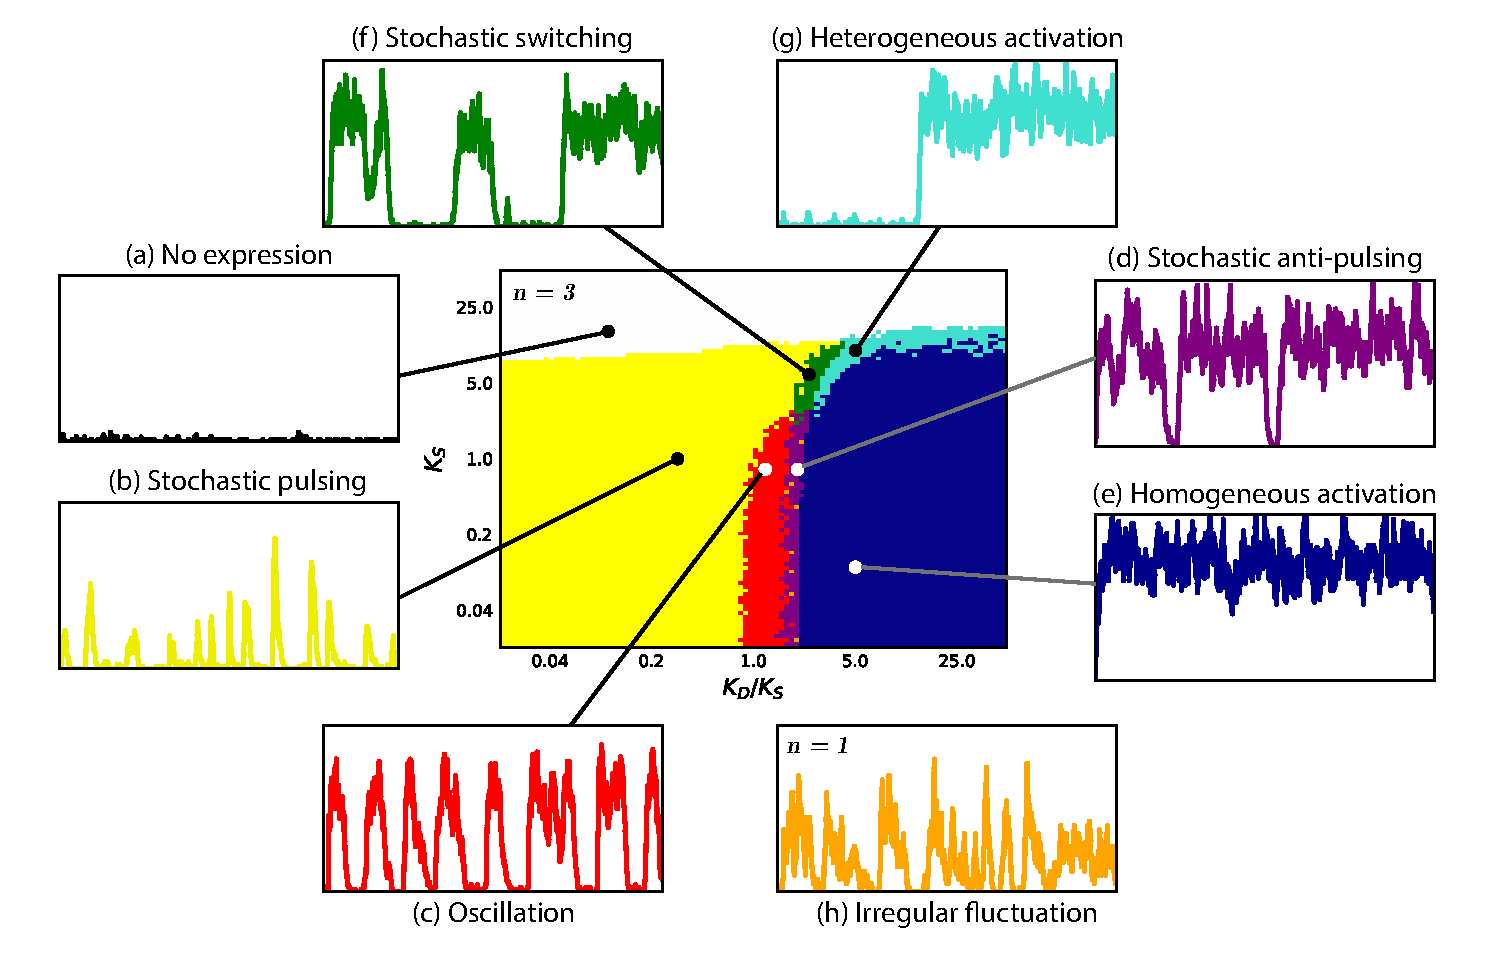
\includegraphics[width = 6in]{different_behaviours.pdf}
    \caption[
        Different dynamical behaviours generated by the mathematical
        model and their mapping to the parametric space
        ]{
        \textbf{Different dynamical behaviours generated by the mathematical
        model and their mapping to the parametric space.}
        (a-g) shows the time-trajectory (x-axis: time and y-axis:
        the amount of sigma factors) of the types of behaviours.
        The trajectory starts immediately after exposure to stress.
        (middle) the types of behaviours mapped to a 
        $K_S$-$K_D/K_S$ parametric space,
        simulated under ultrasensitive Hill coefficient $n = 3$.
    }
    \label{fig:different_behaviours}
\end{figure}

\subsection{Ultrasensitivity is important for bistability and oscillation}
\label{sec:us_for_bs_and_oscillation}

% bistability and oscillations are lost in non-ultrasensitivity
% "ultrasensitivity of the circuit" emphasizes intrinsic ultrasensitivity
To ask what role ultrasensitivity of the circuit plays in its dynamics,
I simulated the range of behaviours across the $K_S$-$K_D/K_S$ 
parametric space with either $n = 1$ (non-ultrasensitive) or
$n > 1$ (ultrasensitive).
%%
The loss of ultrasensitivity significantly changes the landscape
of the behaviour mapping,
with the stochastic anti-pulsing region much expanded and
the oscillation and heterogeneous activation
region completely lost (Figure~\ref{fig:behaviour_mappings_diff_n} A).
%%
A dynamical behaviour is considered stochastic pulsing if 
the abundance of molecules ($\sigma$ and $A$) is attracted to the
ON-state, but large fluctuations persist
(Section~\ref{sec:classification_algorithm}).
%%
Thus, the stochastic anti-pulsing area under $n = 1$ reflects
a range of dynamics that the amount of sigma factors random-walk 
between the ON- and OFF-states without establishing oscillation
or showing bistability.

\begin{figure}[ht]
    \centering
    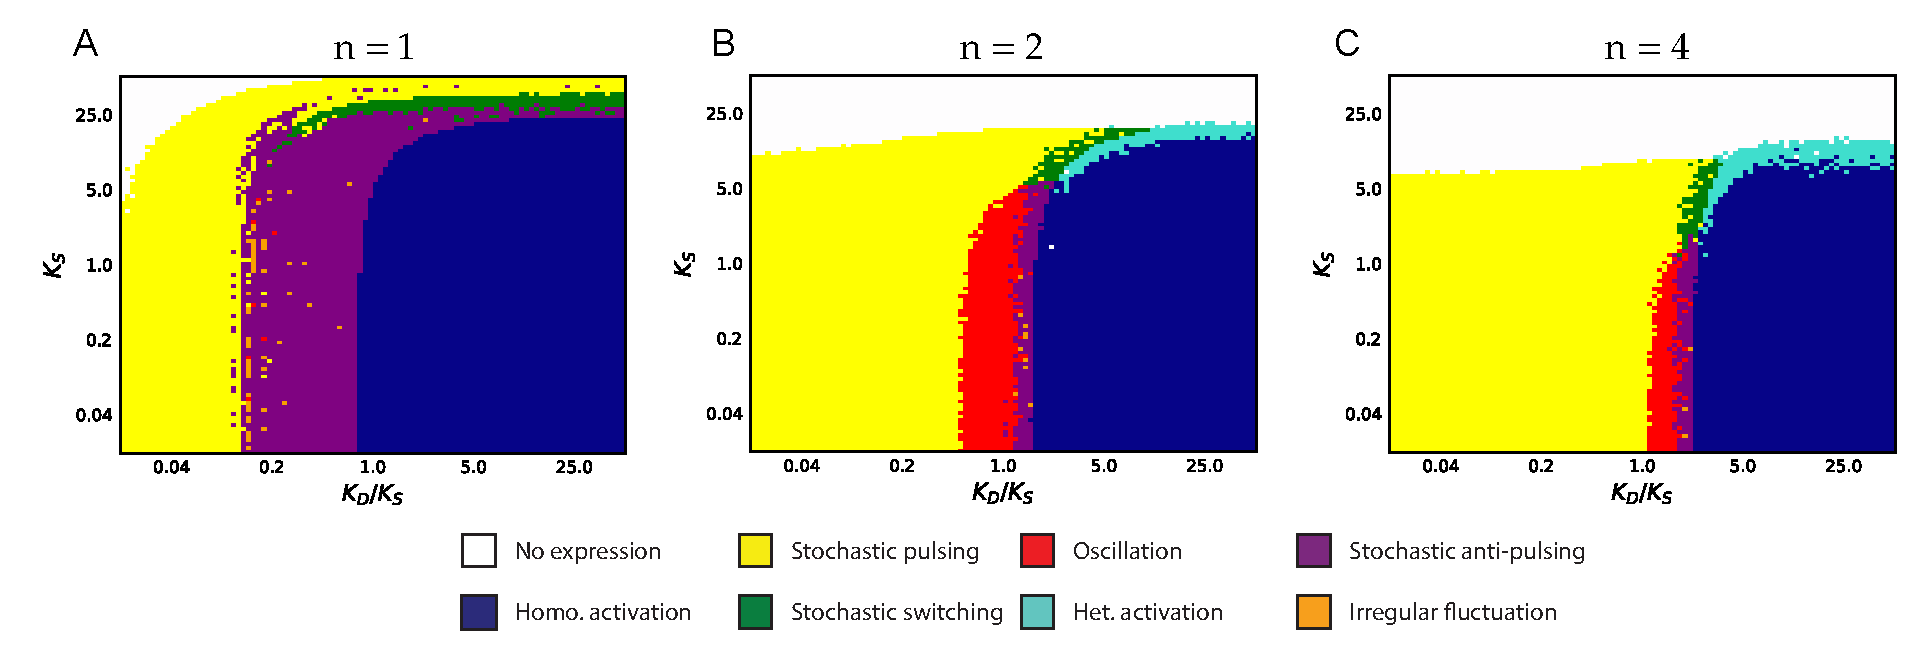
\includegraphics[width = 6in]{behaviour_mappings_diff_n.pdf}
    \caption[
        The mapping of dynamical behaviours across the parametric
        space under different Hill coefficients
        ]{
        \textbf{The mapping of dynamical behaviours across the parametric
        space under different Hill coefficients.} 
        The mathematical model for the alternative sigma factor circuit
        is simulated under three different Hill coefficients
        ($n = 1$, 2 or 4).
        The landscape of the non-ultrasensitive behaviour mapping is
        qualitatively different from the other two.
        $K_S$: the activation threshold (inversely correlated with
        activating strength). $K_D$: the repression threshold (inversely
        correlated with the repressive strength).
    }
    \label{fig:behaviour_mappings_diff_n}
\end{figure}

% why these two behaviours are lost
To explain how some behaviours are lost in the non-ultrasensitive
regime, I examined the non-ultrasensitive counterparts of the
oscillation and stochastic switching dynamics (Figure~
\ref{fig:non_us_counterparts}).
%%
In Figure~\ref{fig:non_us_counterparts},
oscillation (E) and its non-ultrasensitive counterpart (G)
show similar vector fields and the existence of fixed points,
so do stochastic switching (F) and its counterpart (H).
However, their time-dependent trajectories are distinct
from each other.
%%
Under $n = 1$, oscillations collapse into irregular fluctuations,
characterized by no fixed points, but not being periodic either.
%%
Non-ultrasensitivity stochastic switching shows reduced separation
between the ON- and OFF-states and diminished stability of both states.
%%
% Just a possible (intuitive) explanation. Not very confident since no evidence
The lack of ultrasensitivity may promote random walks between
ON- and OFF-states, which makes oscillations and bistability 
difficult to maintain.
%%
% was going to say "intrinsic ultrasensitivity",
% which is a precarious, undefined term
In summary, the loss of ultrasensitivity in the circuit
significantly changes the behaviour mapping across
varying $K_S$ and $K_D$ and makes some behaviours unobtainable.
%%
I showed the importance of ultrasensitivity in maintaining oscillations
and bistability, which is supported by observations of other
genetic circuits \cite{ferrell14c, gardner00c} 
(Section~\ref{sec:biochemical_ultrasensitivity}).
% finally, segue into next section
However, the competition between alternative sigma factors
may be an alternative source of ultrasensitivity that is not accounted 
for in this model of a single sigma factor circuit.

\begin{figure}[ht]
    \centering
    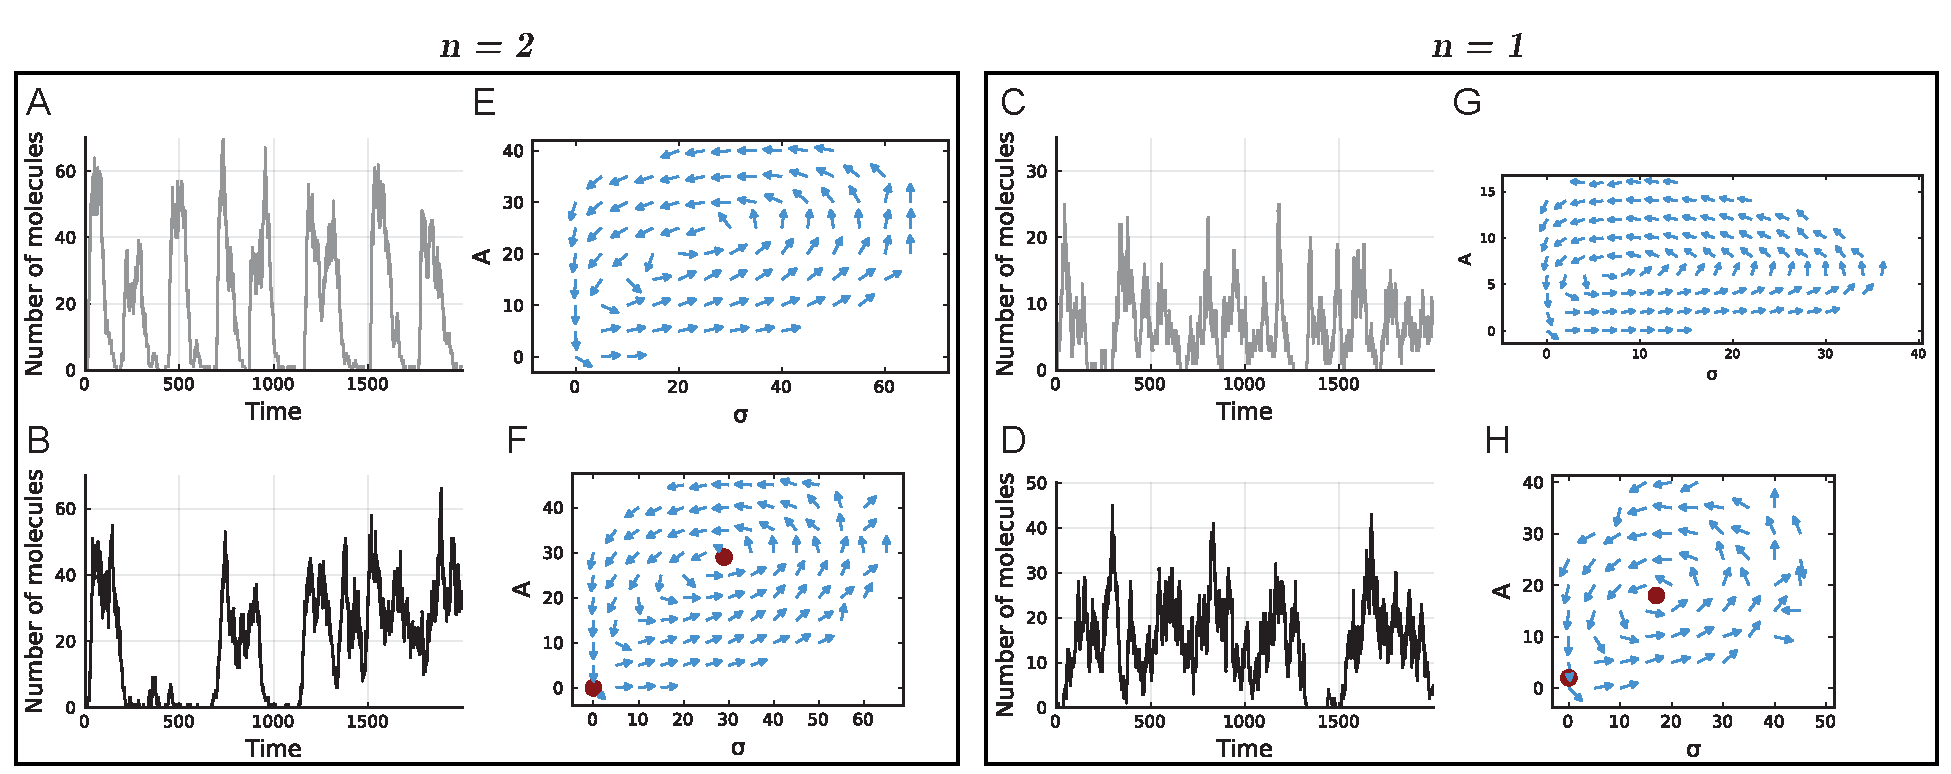
\includegraphics[width = 6in]{non_ultrasensitive_counterparts.pdf}
    \caption[
        The counterparts of oscillation and stochastic switching in 
        non-ultrasensitive regime
        ]{
        \textbf{The counterparts of oscillation and stochastic switching in 
        non-ultrasensitive regime.}
        (A-D) The time-dependent trajectories of 
        oscillation (A) and stochastic switching (B)
        of the ultrasensitive circuit and their counterparts in the
        non-ultrasensitive circuit (C and D).
        The system is exposed to stress at time point 0.
        %%
        (E-H) The corresponding vector field calculated based on
        the trajectories. Red dots mark the fixed points.
        %%
        (A-B and E-F) simulation under $n = 2$, with ultrasensitivity.
        (C-D and G-H) simulation under $n = 1$, without ultrasensitivity.
    }
    \label{fig:non_us_counterparts}
\end{figure}

\clearpage    % some of the figures delay too much
\section{Competition leads to bistability of non-cooperative sigma factor circuit}
\label{sec:competition_to_us}

% why propose new mechanism of ultrasensitivity and how to study it
A previous study shows that \textit{B. subtilis} $\sigma^V$ activates 
heterogeneously upon stress, but there is no known cooperativity 
(thus, also no known source of ultrasensitivity) in the circuit \cite{schwall21a}. 
I have shown that ultrasensitivity is essential for bistable
dynamics, e.g., heterogeneous activation, which suggests that
there could be other source of ultrasensitivity besides binding
cooperativity in the $\sigma^V$ circuit.
Here, I propose new mechanisms (Section~\ref{sec:forced_bistability} and
Section~\ref{sec:both_non_coop_bistability}) 
for the bistability of non-cooperative
alternative sigma factor circuits through the competition of several circuits
for limited RNA polymerase (RNAP) core enzymes.
To validate the mechanisms, I built a mathematical model describing two 
competitive alternative sigma factor circuits and a finite amount of RNAP cores,
where the two sigma factor circuits share the same topology and 
the contribution from the housekeeping sigma factor is reflected by 
the reduced number of RNAP cores (Section~\ref{sec:sigma_competition_model}).

% competitive trajectories show anti-correlations
To visualize the competition between the sigma factors,
I simulated a system of two identical sigma factor circuits, in terms of their
activating/repressive strength and cooperativity, etc., using the
Gillespie algorithm with varying $K_S$ and $K_D$.
The activity of the two sigma factors (in terms of the amount of 
sigma factors bound to the RNAP cores)
show anti-correlations in all of the dynamical behaviours,
including stochastic pulsing, stochastic switching, and activations
(Figure~\ref{fig:time_sharing}).
Depending on the activation threshold ($K_S$), the two sigma factors
can either be activated in parallel (concurrent activation) or the activation 
of one completely repress the other (exclusive activation).
The anti-correlations are important to explain forced bistability
(Section~\ref{sec:forced_bistability}) and,
especially the stochastic switching dynamics here,
represents time sharing activation pattern of the sigma factors,
by which the bacteria may generate heterogeneity in a population 
\cite{schwall21a}.

\begin{figure}[ht]
    \centering
    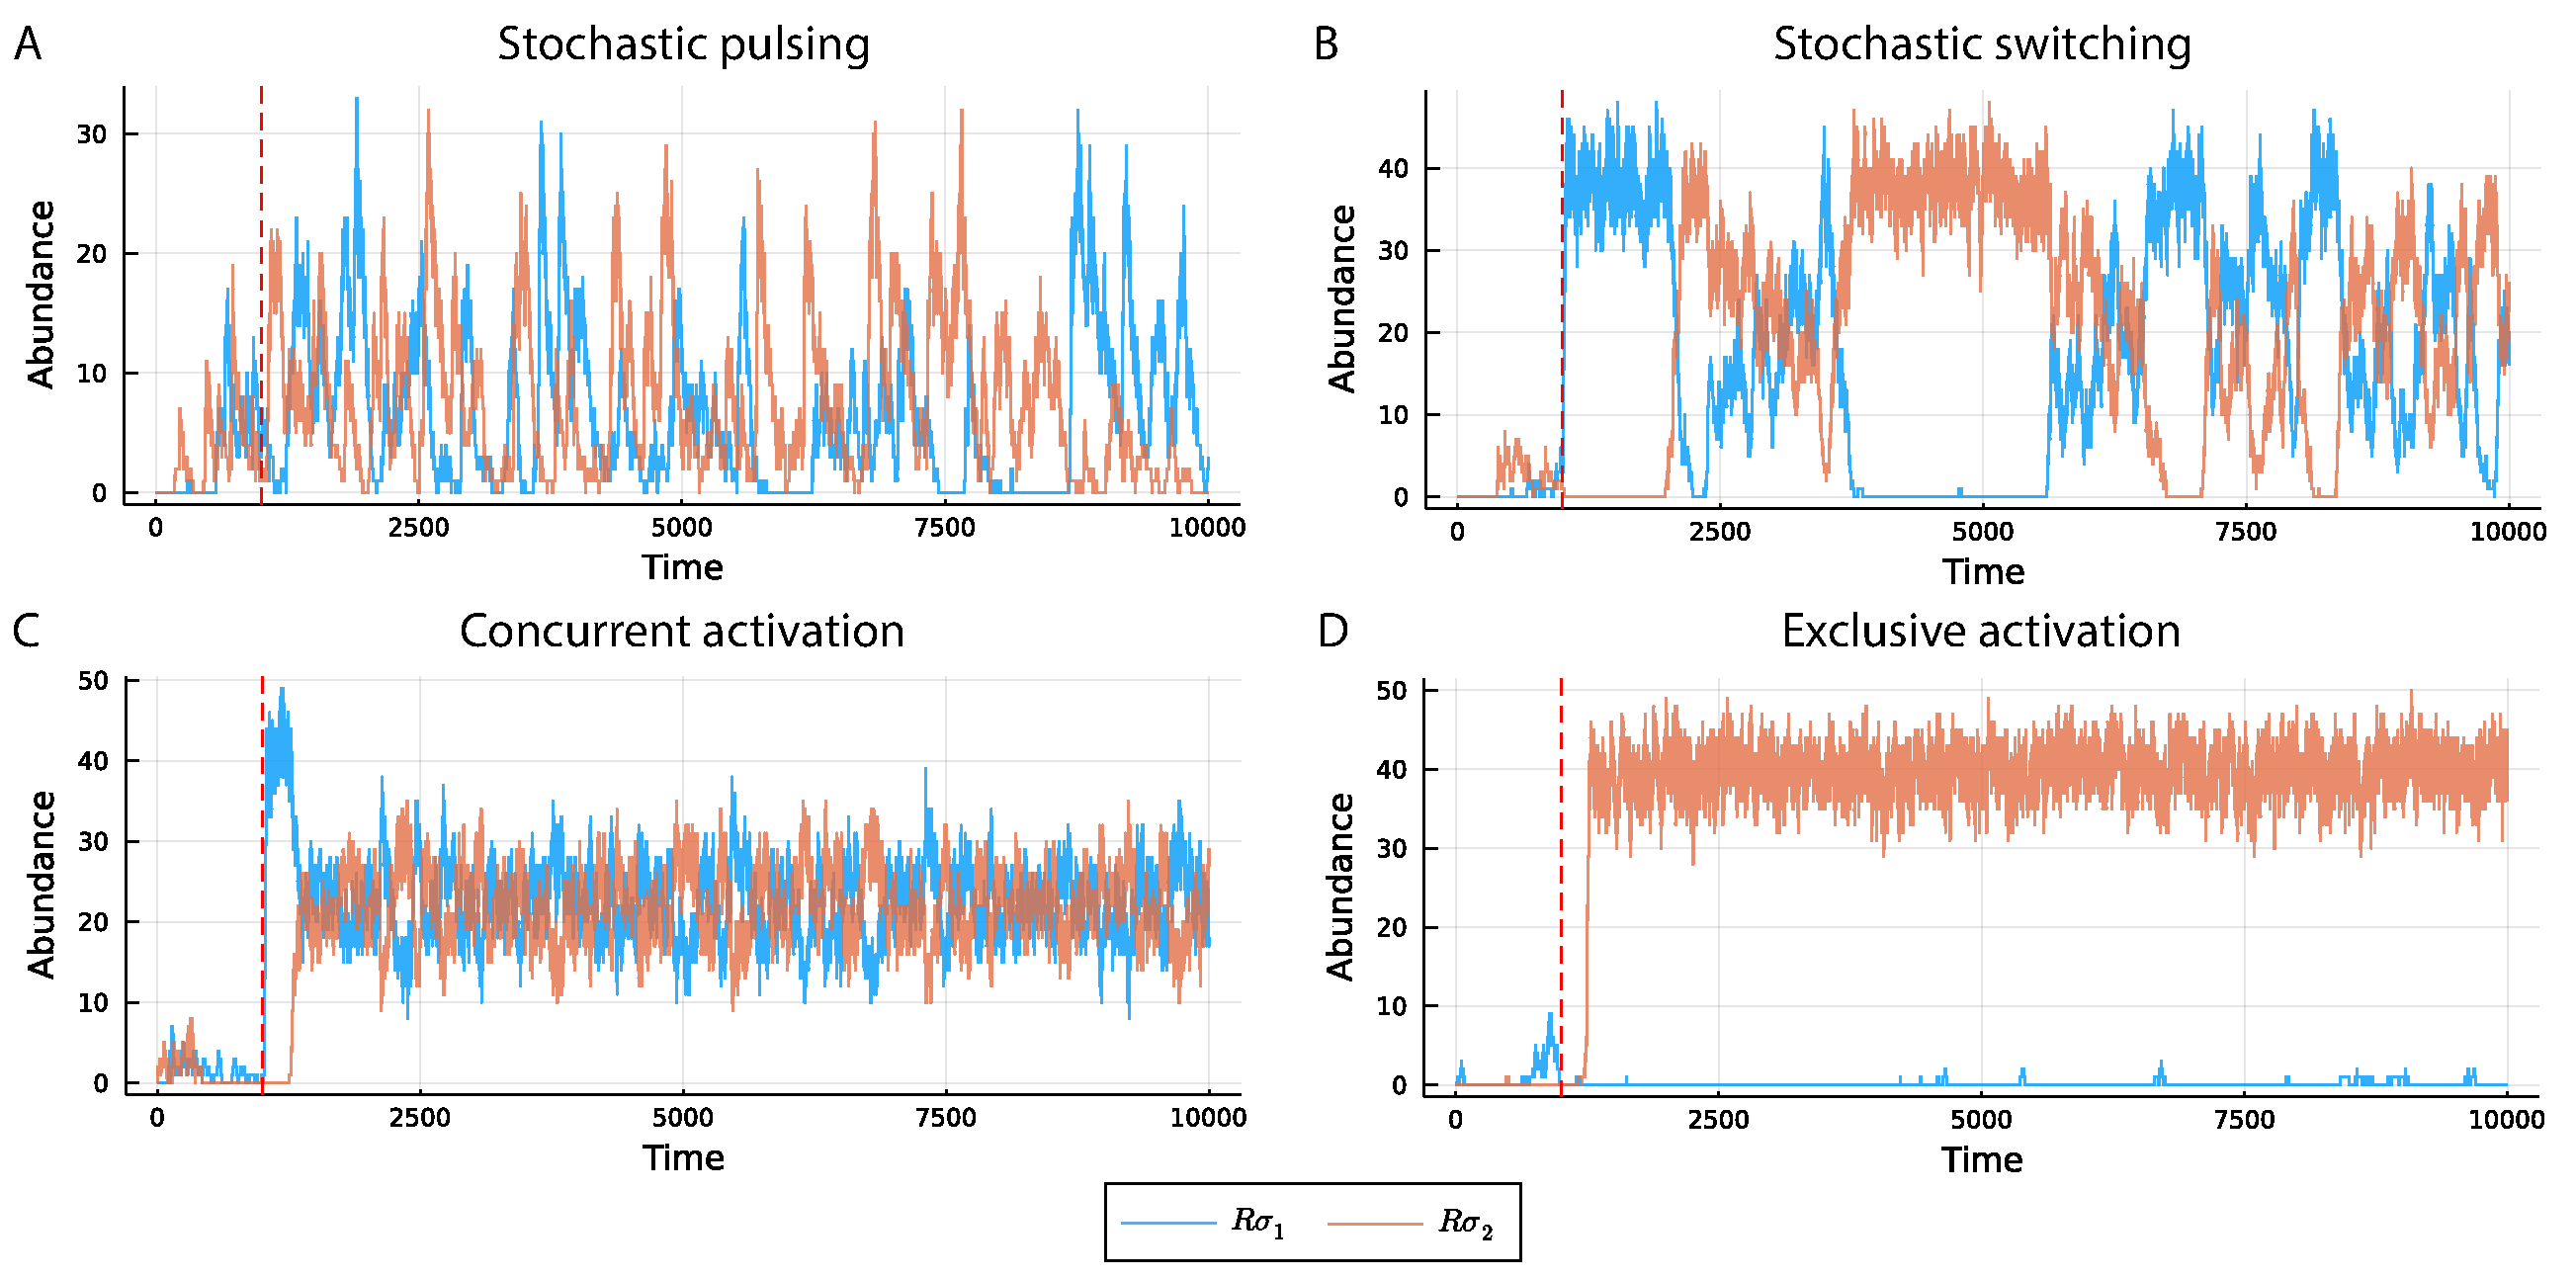
\includegraphics[width = 6in]{time_sharing.pdf}
    \caption[
        Different behaviours of the dual-sigma factor network show
        anti-correlations
        ]{
        \textbf{Different behaviours of the dual-sigma factor network show
        anti-correlations.}
        (A-D) The trajectories of the amount of sigma factors bound
        to the RNAP cores (denoted as $R$), which serves as the activity
        of the sigma factors.
        The total amount of RNAP cores is kept constant at 50.
        The two sigma factor circuits are modelled with the same parameters.
        The red dashed line is the time exposed to stress.
        Binding rate constant between RNAP core and the sigma factor
        $k_1 = 0.005$, the dissociation rate constant
        $k_2 = 0.05$.
    }
    \label{fig:time_sharing}
\end{figure}

\subsection{Forced bistability in asymmetric dual-sigma factor circuits}
\label{sec:forced_bistability}

% forced bistability happens in strong competition
First, I examined a dual-sigma factor competition network where
the Hill coefficients are asymmetric, i.e.,
one of the circuits is without binding cooperativity ($n = 1$, denoted as
$\sigma_1$) while the other one has binding cooperativity
($n = 3$, denoted as $\sigma_2$).
This model represents the actual biochemistry of, e.g., the competition between
\textit{B. subtilis} sigma factors $\sigma^V$ and $\sigma^B$,
since the anti-sigma factor of $\sigma^B$, RsbW, dimerizes and 
cooperatively binds to $\sigma^B$, while the $\sigma^V$ circuit has no known
binding cooperativity \cite{narula16, schwall21a}.
The simulation of the model shows that when the cooperative sigma factor circuit
is in bistable dynamics and when competition is strong,
the non-cooperative sigma factor circuit is forced to be bistable,
while when in weak competition, the dynamics of the cooperative circuit
does not have significant impact on the non-cooperative one
(Figure~\ref{fig:forced_bistability} A).
I suggest that the bistability of $\sigma_2$ causes the amount of free (unbound)
RNAP cores to also switch between high and low states.
Since steady-state expression level of $\sigma_1$ relies on the amount of 
free RNAP cores, it is induced to be bistable.
Unlike $\sigma_2$, the lower state of the non-cooperative $\sigma_1$ bistability
is not necessarily around 0 (Figure~\ref{fig:forced_bistability} B-D).

% forced bistability is stable across k1 and even shows tristability
To ask how the strength of the competition affects the dynamics of the
non-cooperative sigma factor, I simulated the system against different values
of the binding rate constant $k_1$ of $\sigma_1$.
The fixed points are detected as per the classification algorithm
(Section~\ref{sec:classification_algorithm}) and are shown as the 
bifurcation-like diagram (Figure~\ref{fig:forced_bistability} B).
The binding rate constant for the cooperative $\sigma_2$ circuit is fixed.
To keep $\sigma_2$ in bistability, I first examined the region of the
bistable dynamics across the $k_1-K_S$ space (Figure~\ref{fig:k1_KS_mapping}).
Then, the red line is chosen to assign $K_S$ as a linear function of 
$k_1$ across different values of $k_1$ to keep $\sigma_2$ in the bistable regime,
which is $K_S(k_1) = -0.004 \cdot k_1 + 25$.
The bifurcation-like diagram shows that as the hypothetical binding strength
between the sigma factor and the RNAP core increases,
the non-cooperative circuit first transits from the OFF-state to a short
period of bistability, then into tristability (Figure~
\ref{fig:forced_bistability} A middle panel and C).
The tristable dynamics features two non-zero fixed points induced by
the bistable $\sigma_2$ expression and a fixed point at 0 presumably
due to the balance between RNAP holoenzyme formation and sigma
factor degradation (further discussed in Section~\ref{sec:both_non_coop_bistability}).
As $k_1$ of the $\sigma_1$ circuit continues to increase,
the zero fixed point diminishes and the system maintains bistability 
for a rather wide range of parameters.
In summary, in a system of alternative sigma factors competing for a
limited amount RNAP core enzymes, the bistable circuit can force
the non-cooperative circuit to show bistability, or even tristability.

\begin{figure}[ht]
    \centering
    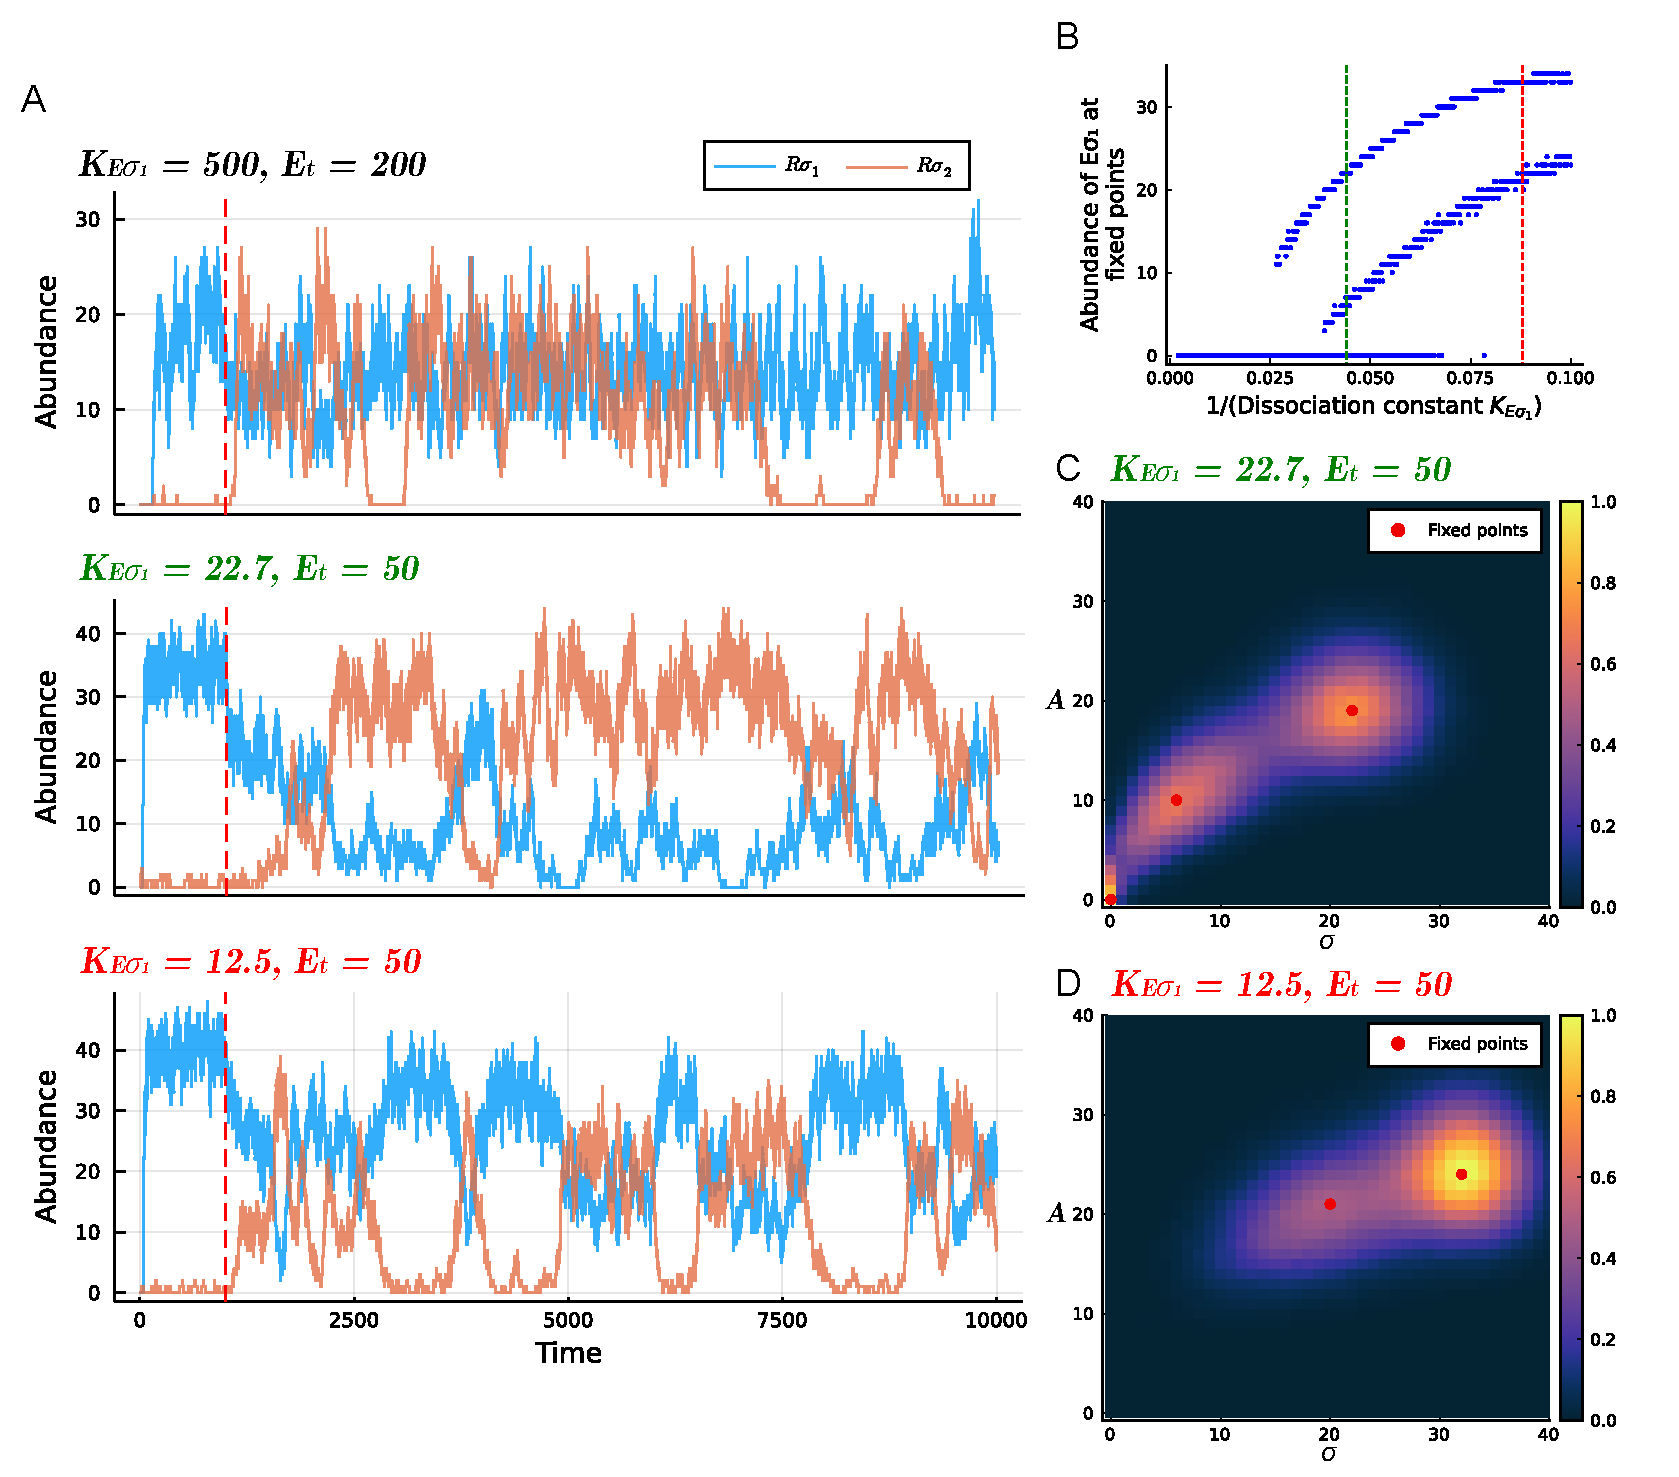
\includegraphics[width = 6in]{forced_bistability.pdf}
    \caption[
        Non-cooperative sigma factor circuit shows forced bistability
        due to the rival bistable circuit
        ]{
        \textbf{Non-cooperative sigma factor circuit shows forced bistability
        due to the rival bistable circuit.}
        (A top) Bistable $\sigma_2$ (cooperative) has no significant 
        influence on the expression of $\sigma_1$ (non-cooperative) under weak
        competition (due to small binding affinity between $\sigma_1$
        and RNAP cores and rather large amount of RNAP cores available).
        (A middle and bottom) the activity of $\sigma_1$ displays forced 
        bistability in strong competition with bistable $\sigma_2$.
        The red dashed line marks exposure to stress.
        $K_{E\sigma_1}$: the dissociation constant of the 
        binding between $\sigma_1$ and the RNAP core ($E$). 
        $E_t$: the total amount of RNAP core enzymes.
        (B) The bifurcation-like diagram of the RNAP core-$\sigma_1$ complex with
        the binding rate constant of $\sigma_1$ as the bifurcation parameter.
        The green and the red dashed line corresponds to the system shown in
        (A middle and C) and (A bottom and D).
        (C-D) The density of the phase paths corresponding to (A middle)
        or (A bottom), respectively showing tristability or bistability.
        $K_{E\sigma_2}$ is fixed at 10 molecules/cell.
    }
    \label{fig:forced_bistability}
\end{figure}

\begin{figure}[ht]
    \centering
    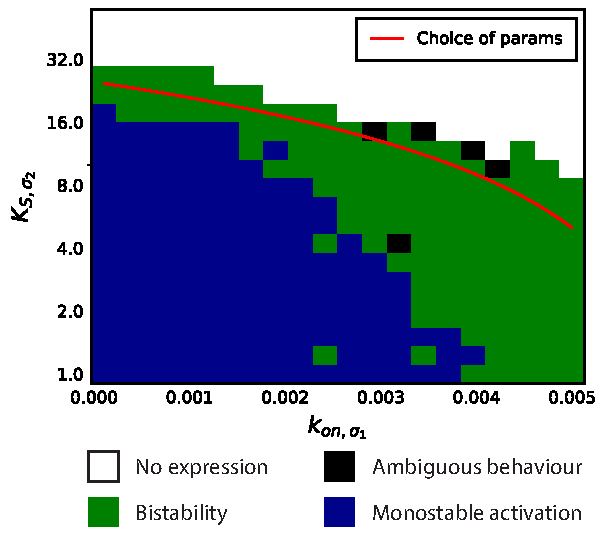
\includegraphics[width = 4in]{k1_KS_mapping.pdf}
    \caption[
        The mapping of the behaviours of non-cooperative sigma 
        factor circuit in the competition model to $k_{on}-K_S$ space
        ]{
        \textbf{The mapping of the behaviours of non-cooperative sigma 
        factor circuit in the competition model to $k_{on}-K_S$ space.}
        The red line shows the function of $K_S$ given $k_{on}$ to keep
        the cooperative sigma factor circuit in bistability, especially,
        $K_S(k_{on}) = -0.004 \cdot k_{on} + 25$.
        $k_{on}$: the binding rate constant of the non-cooperative sigma
        factor. $K_S$: the activation threshold of the cooperative circuit.
    }
    \label{fig:k1_KS_mapping}
\end{figure}

\clearpage
\subsection{Non-cooperative bistability arises from low binding affinity}
\label{sec:both_non_coop_bistability}

Here I explored the situation where none of the sigma factor circuits
in the system are cooperative.
%%
Using the dual-sigma factor competition model with the Hill coefficient
of both circuits set to one, I found a new bistable behaviour with
an almost strict-zero OFF-state and a fluctuating ON-state
(Figure~\ref{fig:strict_zero_bistability} A).
%%
The bistability only holds when (\textit{a}) the amount of available
RNAP cores are limited, and (\textit{b}) the binding affinity between
sigma factors and RNAP cores is considerably low,
%%
e.g., the trajectory in Figure~\ref{fig:strict_zero_bistability} A is 
simulated under $E_t = 50$ and $K_{E\sigma} = 80$
(units: molecules per cell).
%%
In comparison, the binding affinity for the non-ultrasensitive sigma
factor in forced bistability is moderate $K_{E\sigma_1} = 10$
(for parameter specifications see Section~\ref{sec:discussion_parameters}).
%%
The dynamics of the rival sigma factors have no significant effect
on each other (data not shown), which could be the consequence
of low binding affinity.
To reflect this, all simulations that contribute to 
Figure~\ref{fig:strict_zero_bistability} are made with one of the 
sigma circuits turned off.
%%
The density of the occupancy of RNAP cores is clearly bimodal,
with the first peak at zero (silenced) and the second one
around 10\%, which reflects the low binding affinity
(Figure~\ref{fig:strict_zero_bistability} B).
%%
As the relative strength of activating force increases,
the dynamics of the circuit transitions from stochastic switching
to heterogeneous activation (Figure~\ref{fig:strict_zero_bistability} C).
%%
Multiple trajectories in Figure~\ref{fig:strict_zero_bistability} C
simulates a genetically identical bacterial population displaying
heterogeneity in terms of the start of stress response.
%%
Based on the trajectories I plotted the accumulated fraction of
activation in the population.
I found that the variability of
the start of the activation reduces against increasing binding
affinity $K_{E\sigma}$ (Figure~\ref{fig:strict_zero_bistability} D).
%%
Such observation also supports that the weak binding between
sigma factors and RNAP cores accounts for heterogeneous activations.
%%
As the OFF-states feature strict zero-amount of $E\sigma$ complex,
one hypothesis of the mechanism of bistability is that
the low abundance of $E$ and the low affinity of $\sigma$ to it
combined makes the production of a single holoenzyme very rare.
Due to the positive autoregulation of the sigma factor,
the formation of a single holoenzyme can switch on the circuit and
then, it is turned off by random fluctuations.
%%
In summary, I found that in a regime of low RNAP core availability
and low binding affinity of sigma factors to the cores,
sigma factor dynamics exhibits bistability.
This new mechanism may address the activation heterogeneity
of the non-cooperative $\sigma^V$ circuit in \textit{B. subtilis},
and may represent a general mechanism for the generation of 
dynamics that require ultrasensitivity from a non-cooperative circuit.

\begin{figure}
    \centering
    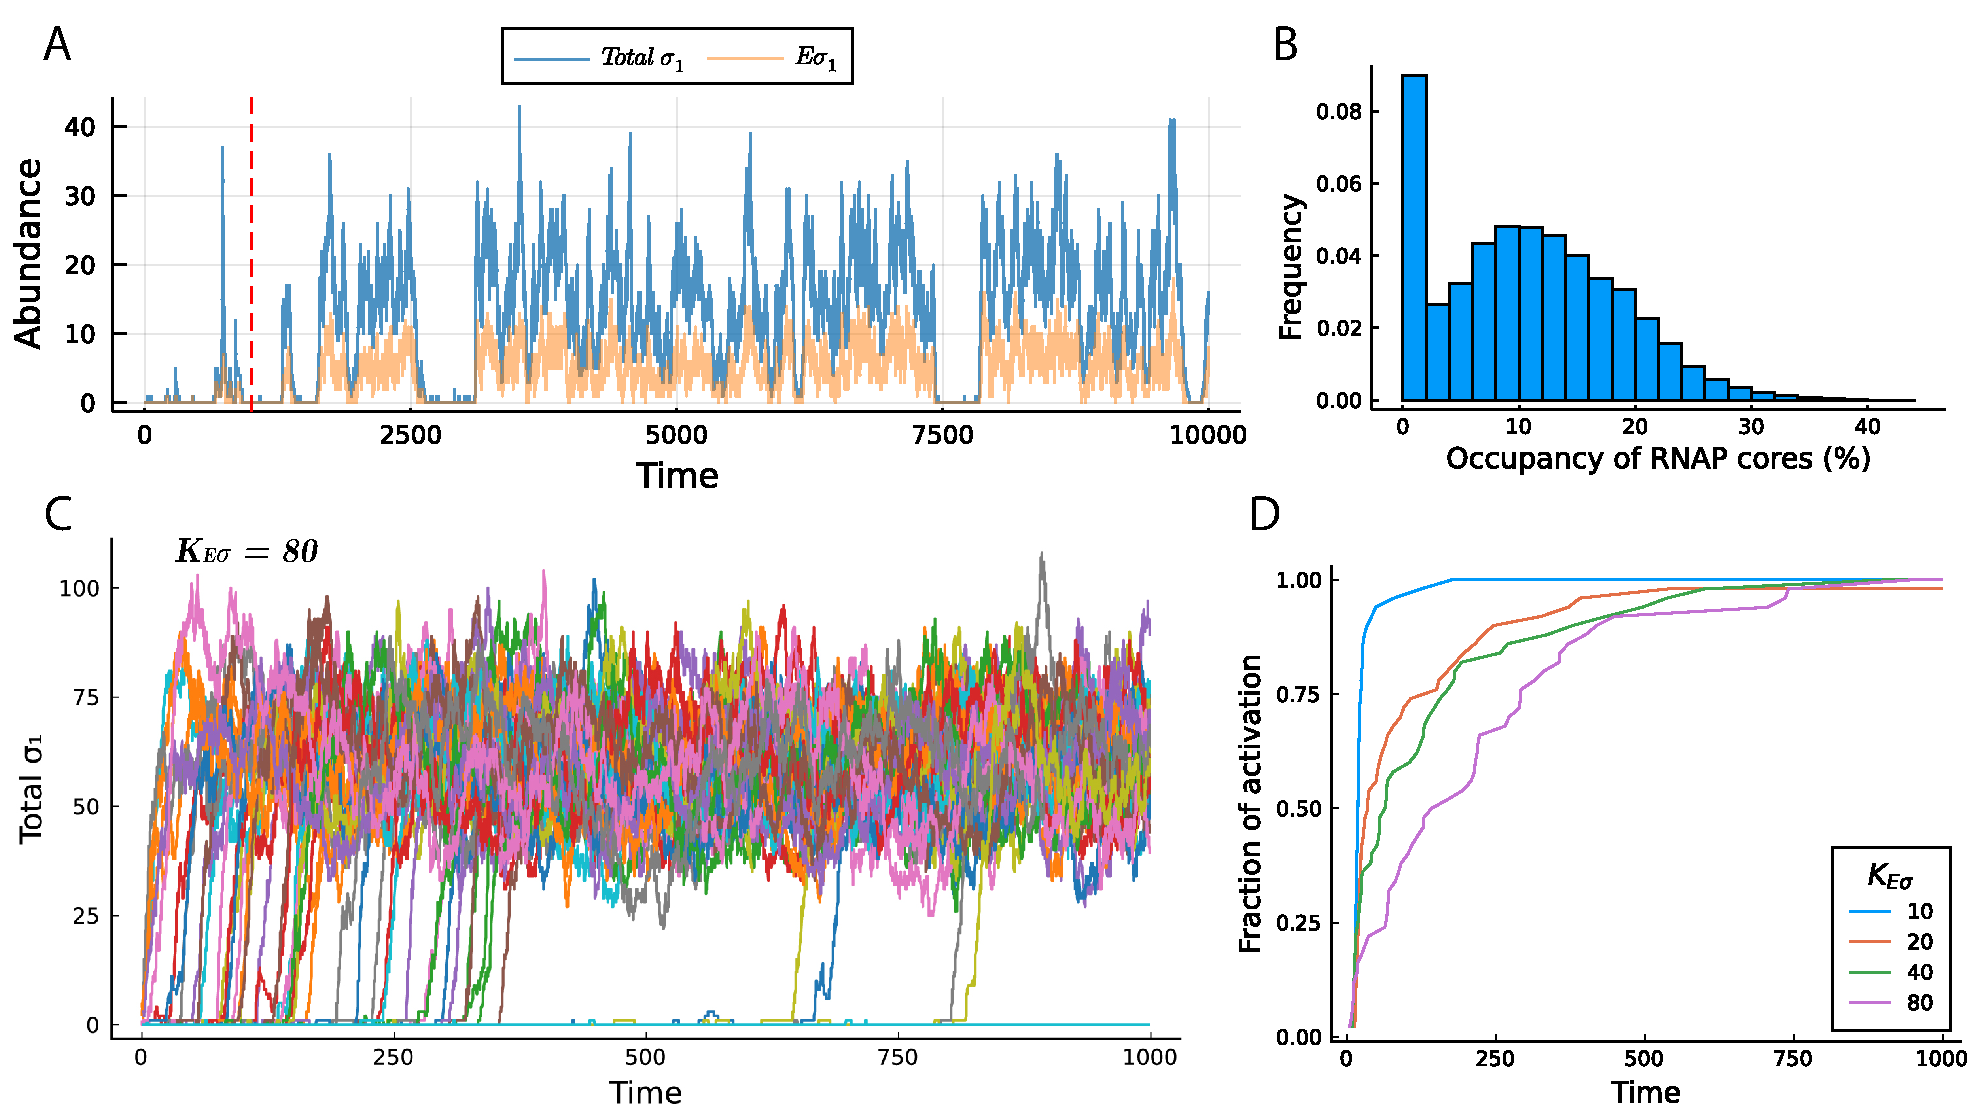
\includegraphics[width = 6in]{strict_zero_bistability.pdf}
    \caption[
        The bistable dynamics of non-cooperative alternative sigma factor
        circuit under low RNAP core affinity
        ]{
        \textbf{The bistable dynamics of non-cooperative alternative sigma factor
        circuit under low RNAP core affinity.}
        (A) Trajectories of total sigma factors and the bound
        sigma factors. The dashed red line indicates exposure to stress.
        In the simulation, $K_{E\sigma} = 80$ and $K_D/K_S = 0.22$.
        (B) Distribution of the occupancy ratio of RNAP cores by sigma factors
        cumulated along the time course of the simulation.
        The distribution is bimodal, which centers at 0 and around 10\%.
        (C) Trajectories of total sigma factors from 50 repeated simulations.
        In the simulation, $K_{E\sigma} = 80$ and $K_D/K_S$ is increased to 0.5
        to stabilize the activation state.
        (D) Accumulated fraction of activation across different binding affinity,
        where activation is defined as the time when
        the amount of sigma factors reaches ON-state.
    }
    \label{fig:strict_zero_bistability}
\end{figure}
%!TEX root = ../thesis.tex
%*******************************************************************************
%*********************************** Fourth Chapter *****************************
%*******************************************************************************

\chapter{Discussion}  %Title of the First Chapter

% \ifpdf
%     \graphicspath{{Chapter1/Figs/Raster/}{Chapter1/Figs/PDF/}{Chapter1/Figs/}}
% \else
%     \graphicspath{{Chapter1/Figs/Vector/}{Chapter1/Figs/}}
% \fi


%********************************** %First Section  **************************************
\section{Considerations on the model}

%% a bit context
The change of environment can be drastic and frequent considering
small size of bacteria,
which often demands the use of alternative sigma factors to adapt
to the new environment through a shift in the transcription profile.
%%
It is established that bacteria leverage noise to dynamically modulate
the expression of sigma factors and, thus, create phenotypic
heterogeneity inside the population to gain a survival advantage
\cite{locke11,cabeen17,park18a,schwall21a}.
%%
Theoretical studies show that a common network motif combining 
a positive autoregulation and a negative feedback loop with delay
underpins these dynamics (\cite{schwall21a} and Torkel Loman's
unpublished work).
%%
% mechanistic, implies bottom-up (though the parameters are
% biochemically explicable, I'm not confidence in their accuracy)
In this study, I used a simplified, mechanistic model of the same 
general structure to reproduce diverse dynamical behaviours of
the sigma factors.
%%
I used the discrete Gillespie algorithm to correctly predict the 
low-molecule dynamics and properly reflect the role of noise
in the circuit.
%%
I also proposed two new mechanisms to address the bistability
suggested in non-cooperativity circuits \cite{schwall21a}
through competition, namely
%%
(\textit{a}) A competing cooperative sigma factor circuit forces
bistability via shared pool of RNAP.
%%
(\textit{b}) Bistability in a non-cooperative circuit
maintained by rare sigma factor-RNAP core
binding event due to low binding affinity.
%%
The theoretical work here could motivate future studies to alter the 
sigma factor-RNAP core binding affinity (e.g. via sigma factor mutants)
to discover potential new dynamical behaviours.
%% 
It may also provide new insights for synthetic biologists to engineer
new oscillators or bistable switches by rewiring the 
bacteria sigma factor circuits.
%%
Nonetheless, the model is built under considerable uncertainty of the
actual biochemical processes and trade-off between generality
and the amount of molecular details encoded.
%%
% this is a strange sentence. Behind is some degree of diffidence,
% nevertheless, it is difficult to gather the last pieces together
Here, I will elaborate some important decisions and assumptions
for the model, and several future directions.

\subsection{Arbitrary units of time}
\label{sec:arbitrary_units_time}

Although the model uses the absolute, discrete number of molecules
per cell as the concentration for all chemical species
to accurately account for stochastic fluctuations,
the units of time are arbitrary.
%%
Notice that in the model (Section~\ref{sec:low_CN}),
the maximum steady-state concentration and the molecular lifetime
is tuned independently through $\beta$ and $\tau$.
%%
When the circuit is activated, the expression rate factor $v_H$ is 
high and can approximate to 1.
Thus, the steady-state abundance of $\sigma$ is roughly $\beta$.
%%
% establish that \tau is the average lifetime
The degradation rate $1/\tau$ gives the molecule an average lifetime
of $\tau$. To support the argument, consider the (deterministic) first-order 
degradation reaction of molecule $x$ with degradation rate constant
$1/\tau$:

\begin{align}
    \frac{dx}{dt} = -\frac{1}{\tau}\cdot x
\end{align}

Given the initial concentration $x_0$ at $t = 0$, the evolution of $x$
along time is expressed as

\begin{align}
    x = x_0 \cdot e^{-t/\tau}
\end{align}

When $x_0$ is large enough, the average molecular lifetime ($\bar{t}$) can be 
approximated by the area under the $t$-$x$ curve divided by the
total number of molecules, $x_0$, namely

\begin{align}
    \bar{t} =& \frac{1}{x_0}\int_{t = 0}^{\infty}x_0 e^{-t/\tau}dt\\
        =& \tau
\end{align}

Which shows that in first-order degradation kinetics, the reciprocal
of the degradation rate is the average molecular lifetime.

In the model, time is measured relative to the average lifetime of
different molecules.
In all simulations, the lifetime of the sigma factor is 10 time units.
To reflect the delay from the anti-sigma factor, the lifetime of
$A$ is set to 50, 5-times of that of the sigma factor.
%%
% validate k_off
In the case of competition against the RNAP cores,
the dissociation rate constant $k_{off}$ is reported to be 
\SI{1e-3}{\per\second}, equivalent to the average lifetime
of $E\sigma$ being \SI{1000}{\second} \cite{mauri14}.
%%
The average lifetime of sigma factors is required to normalize
$k_{off}$ to the time units I use.
To begin with, the half-life of the major pool of proteome in $E. coli$ 
is reported to be around 1 hour.
From first-order degradation kinetics, we can derive that half-life
is $\ln 2 \cdot \tau$ (proof not shown) and thus,
the average lifetime is around \SI{5000}{\second} \cite{maurizi92}
%%
However, another study reports the half-life of bacteria sigma factor
under protease negative regulation to be 1 minute, 60-times faster than
the average proteome \cite{el-samad05}.
%%
Given the scarcity of measurement, I approximately set the average lifetime
of the holoenzyme to be the same as sigma factor (\SI{1000}{\second}).
%%
% finally, how to improve
The predictability of the model can be improved by dedicated measurements
of the half-lives of the holoenzyme and the sigma factor.
%%
Also, altering the relative lifetime of the anti-sigma factor compared
to the sigma factor could reveal interesting dynamics,
which contributes to future research directions.
%%
However, I argue that the accuracy of the simulation is not harmed
by the use of arbitrary time units, since I inspected that
the change of absolute lifetime of molecules does not change the 
steady-state distribution of sigma factors, given a small
time step used (data not shown).

% \subsection{Steps of reaction under steady-state assumptions}
\subsection{Derivation of model parameters}
\label{sec:discussion_parameters}

In this section, I will discuss the rationale of choosing other
model parameters besides the aforementioned degradation/dissociation
rates.
%%
% the dissociation constant is important
The dissociation constant between RNAP cores and sigma factors,
$K_{E\sigma}$, quantifies the binding affinity and plays an important
role in tuning the strength of sigma factor competition and,
thus, the existence of bistability in the system.
%%
The dissociation constant has the units of concentration
\cite{alon06}.
Since I used molecules per cell as the units for concentration
as many literature report dissociation constants in 
molar concentrations,
I will first determine the conversion between the two.
%%
% conversion between molar and molecules
% warning: the style of siunitx is a bit weird
Nanomolar (\si{\nano\Molar}) is the common units for the 
physiological concentrations of macromolecules.
Multiplying the unit concentration (\SI{1}{\nano\Molar}) by the average cellular
volume of bacteria (\SI{1.32}{\femto\liter}) \cite{mauri14} and the
Avogadro constant gives approximately 0.8 (molecules/cell).
%%
Maeda \textit{et al.} reported that the dissociation constants
of the alternative sigma factors in \textit{E. coli} range from
\SI{0.3}{\nano\Molar} to \SI{4.26}{\nano\Molar}, which translates to
0.24 to 3.41 molecules/cell \cite{maeda00}.
%%
However, a more recent study measures the binding affinity
by a different method in various cellular conditions.
The study displays that the dissociation constant
between one of the sigma factors, RpoH (alias $\sigma^H$ or $\sigma^{32}$) 
and RNAP cores
may range from 18 to 100 molecules/cell across different temperatures 
\cite{ganguly12}.
%%
Though both studies consistently report the binding affinity to
the housekeeping sigma factor to be higher than any of the alternative
ones, the absolute values can vary 10- to 100-fold, depending on
different methods and measuring conditions.
%%
I chose $K_{E\sigma}$ between 10 to 100 molecules/cell for most simulations,
in comply with the newer measurements.
%%
Notice that both studies measure the dissociation constants 
\textit{in vitro}. It would be interesting to see \textit{in vivo}
measurements, which may solve the conflicts and improve model accuracy.
%%
Also, since the $E$-$\sigma$ dissociation constant is shown to
change according to ionic strength and temperature.
Future study may explore whether the change in binding affinities
contribute to sigma factor competition.

% Finally, we talk about the amount of RNAP cores and 
% housekeeping sigma factors
The concentration of RNAP core enzyme in bacteria is also
an unsettled case, with estimates ranging from
approximately 1,500 to 13,000 copies per cell \cite{jishage95,grigorova06}.
%%
To ask the proportion of RNAP cores associated with
the alternative sigma factors, which is the number used in the model
to reflect housekeeping sigma factor competition,
I designed an equilibrium binding model.
%%
The total number of RNAP enzyme cores is set to $E_t = 2,000$.
Since the amount of housekeeping sigma factors (denoted by $\sigma^A$)
is reported to significantly exceed at approximately 3-fold,
I set $\sigma^A_t = 6,000$.
Finally, I chose the number of all alternative sigma factors to be
$\sigma^B_t = 2,000$ to reflect the observation that the alternative
sigma factors are fewer than the housekeeping ones.
%%
From the above discussion of binding affinities, I set
$K_{E\sigma^A} = 1$ and $K_{E\sigma^B} = 10$ to show the weaker 
binding affinities of the alternative sigma factors.
%%
The model is given by:

\begin{gather}
    K_{E\sigma^A} = \frac{E \cdot \sigma^A}{E\sigma^A}\\
    K_{E\sigma^B} = \frac{E \cdot \sigma^B}{E\sigma^B}\\
    E_t = E + E\sigma^A + E\sigma^B\\
    \sigma^A_t = \sigma^A + E\sigma^A\\
    \sigma^B_t = \sigma^B + E\sigma^B
\end{gather}

Where $E$ represents only the free RNAP cores, while $E\sigma^A$
are the ones bound to the housekeeping sigma factors,
and $E_t$ is the total amount.
The sigma factors adopt the same rules of notations.
%%
Solving the equations gives almost saturated RNAP core binging,
with $E\sigma^A \approx 1,910$ and $E\sigma^B \approx 89$
(molecules/cell).
%%
In the core model for the sigma factor circuit,
I used a smaller $E = 50$ (RNAP cores available to alternative 
sigma factors) in most settings
to simulate a fierce competition scenario.
%%
Altering the amount RNAP cores available to the alternative sigma
factors is shown to weaken the competition 
(Section~\ref{fig:forced_bistability}).
Future study may further quantify the effects and explore
whether bistability can sustain with changing total number of RNAP cores.

\section{Future work}

By simulating a simplified two-component mathematical model
of the alternative sigma factor circuit, I produced a range of
behaviours, some of which have been experimentally observed.
%%
From this model, I examined the scenario where two alternative sigma
factor circuits compete for the limited amount of RNAP cores.
From there I discovered two new bistable patterns of 
the sigma factor circuit.
%%
First, when the binding between sigma factors and RNAP cores
is strong, and if a ultrasensitive circuit exists in the cell,
another non-ultrasensitive circuit can be induced to be bistable.
The bistability could be transferred through the shared, limited
pool of RNAP cores.
%%
Second, when the binding affinity is weak (and if the amount of 
RNAP cores are limited due other sigma factors, especially
the housekeeping one), the event of holoenzyme formation may be
rare. Then, the system would be turned on by the rare binding event
and be turned off due to random walk to zero from a relative small number
of holoenzymes.

Considering that the research is theoretical, it would
be strengthened by evidence from experiments.
Furthermore, several experimental observations may provide the
model with new insights and in turn refine the theory.
%%
To begin with, there are still a few interesting directions that
one may explore under the current modelling framework.
%%
First, since the Gillespie algorithm generates correct low-copy number dynamics, 
it would be interesting to ask what is the effect of absolute 
number of molecules in the system to different dynamical behaviours.
%%
Experiments have shown that when noise is reduced due to an
increase in the absolute number of molecules, some dynamical 
behaviours, e.g., stochastic switching and stochastic pulsing,
can be weakened \cite{suel06, locke11}.
%%
It would be important to validate and quantify this effect in theory.
%%
Second, I observed that, similar to the effects of ultrasensitivity,
tuning the molecular lifetime of the anti-sigma factor to be
less than that of the sigma factor eliminates some behaviours,
including oscillation (data not shown).
%%
Intuitively, since the lifetime of anti-sigma factors determines the
time delay of the negative feedback in the model and the lifetime
of sigma factors determine the speed of positive autoregulation,
establishing the oscillation may require a relative slower
negative feedback.
%%
It will be interesting to confirm this from simulation or theory.

Several experiments may strengthen the foundation of the model,
including measuring the average lifetime of different sigma factors
(considering both protein degradation and dilution effects)
and the dissociation rate of the holoenzyme.
%%
A more important aspect is to measure the sigma factor-RNAP core
binding affinity (in the form of dissociation constant 
$K_{E\sigma}$) \textit{in vivo},
since this binding affinity has major implications to sigma factor
behaviours under competition.
%%
Moreover, there is still huge uncertainty in its measurement,
which is complicated by the dependence of $K_{E\sigma}$ on
different cellular conditions (Section~\ref{sec:discussion_parameters})
\cite{ganguly12}.
%%
Future research may pivot on whether stress influences the binding
affinity and, thus, alters sigma factor dynamics.
%%
The behaviour mapping in Figure~\ref{fig:different_behaviours}
predicts several dynamical behaviours of sigma factors that have
not yet been experimentally observed,
e.g. oscillation, stochastic anti-pulsing, etc.
%%
It would be possible to observe these behaviours using single-cell
techniques, by either constructing sigma factor or anti-sigma factor
mutants, or simply by tuning the strength of stress.
%%
The model also suggests that the strength of competition can modify
the bistable dynamics of non-ultrasensitive sigma factors.
%%
Relevant experiments can not only serve as a confirmation of the proposed
molecular mechanisms, but also help to discover new ways to tune
the phenotypic variability of a bacterial population.
%%
For example, the strategy which \textit{B. subtilis} tunes the variability
of $\sigma^V$ by the strength of stress is qualitatively reproduced by my model
\cite{schwall21a}.
%%
Finally, the range of dynamical behaviours shown in sigma factors may 
contribute to the synthetic biology toolbox.
%%
Orthogonal sigma factor circuits from other species
can be leveraged as a frequency-tunable stochastic pulsing generator
or as a source of heterogeneity in a population.

% \subsection{Heterogeneous activation time of sigV}
% \subsection{Transient single pulsing of sigB}

%!TEX root = ../thesis.tex
%*******************************************************************************
%*********************************** Fifth Chapter *****************************
%*******************************************************************************

\chapter{Conclusion}  %Title of the First Chapter

% \ifpdf
%     \graphicspath{{Chapter1/Figs/Raster/}{Chapter1/Figs/PDF/}{Chapter1/Figs/}}
% \else
%     \graphicspath{{Chapter1/Figs/Vector/}{Chapter1/Figs/}}
% \fi


%****************all in one section*********************

Noise unavoidably arises from the thermal motion of molecules and
from the fluctuating environment where the cells reside.
However, more and more evidence has shown that noise may play functional
role in biology \cite{raj08,eldar10a}.
%%
Bacteria can utilize noise to activate a specific set of genes
in a fraction of the population to create phenotypic 
heterogeneity.
%%
In this way, bacteria may "hedge their bets" to make some individuals
survive a sudden change in the environment or benefit the individuals
that do not switch on stress response (thus less metabolic burden)
if the favourable environment recovers
(Section~\ref{sec:functional_role_noise}).
%%
In bacteria, the activation of a certain group of genes is typically directed
by the expression of alternative sigma factors.
%%
Previous studies have shown that sigma factors may exhibit dynamical
behaviours upon stress, e.g. stochastic pulsing ($\sigma^B$ of
\textit{B. subtilis}) and heterogeneous start of activation
($\sigma^V$ of \textit{B. subtilis}) \cite{locke11,schwall21a}.
%%
In this study, I simulated a simplified mechanistic model 
with the Gillespie algorithm and produced
a wide range of behaviours, e.g., stochastic pulsing, stochastic
state-switching, stochastic anti-pulsing (i.e. inactivation pulsing),
oscillation, etc (Section~\ref{sec:general_diff_behaviours}).
%%
The model features mixed positive autoregulation and negative 
feedback loop (\cite{schwall21a} and Torkel Loman's unpublished work)
(Section~\ref{sec:low_CN}).
%%
Biochemical ultrasensitivity has been shown to facilitate some
dynamical behaviours, including oscillation and stochastic state-switching
\cite{ferrell14c}.
%%
However, the role of ultrasensitivity in the alternative sigma factor 
circuit remains unclear.
%%
By simulating a non-ultrasensitive circuit ($n = 1$), I observed that
not only is oscillation lost, but also other behaviours, 
e.g. stochastic switching and stochastic anti-pulsing, are significantly
weakened by increased fluctuations
(Section~\ref{sec:us_for_bs_and_oscillation}).
%%
Though ultrasensitivity can be important for bistability,
many sigma factor circuits show no known source of ultrasensitivity
from binding cooperativity.
%%
This suggests that there can be other sources of ultrasensitivity.
%%
It has also been shown that sigma factors are in competition with each
other for the limited amount of RNAP cores 
(Section~\ref{sec:intro_sigma_competition}).
%%
In light of that, I simulated a dual sigma factor model to reflect
the competition between them (Section~\ref{sec:sigma_competition_model}).
%%
Based on the model, I proposed two new mechanisms for bistability to
emerge from a non-ultrasensitivity circuit.
%%
First, when competition is strong, one ultrasensitive, bistable sigma factor
circuit can force another non-ultrasensitive circuit to show
bistability through the limitation of a shared pool of RNAP cores
(Section~\ref{sec:forced_bistability}).
%%
Second, when the binding affinity between the non-ultrasensitive
sigma factor and the RNAP core is low,
the abundance of sigma factors is trapped in a strict-zero state.
The circuit is then turned on by rare binding events and turned off
by the random walk from a low copy number to zero
(Section~\ref{sec:both_non_coop_bistability}).
%%
In the second scheme, I also showed that the activation variability caused by
bistability increases as the binding affinity decreases,
which qualitatively reflects the observations of $\sigma^V$ in 
\textit{B. subtilis} \cite{schwall21a}.
%%
As the core structure used in the model is shared among various bacterial
alternative sigma factor circuits,
these mechanisms may represent a general strategy to generate 
heterogeneity in a population.
%%
In future studies, it would be interesting to experimentally explore other
dynamical behaviours predicted by the model.
%%
It would also be important to validate the proposed mechanisms of 
non-ultrasensitive bistability by experiments.
%%
Finally, considering the wide range of dynamics produced from the
rather simple sigma-anti-sigma circuit, engineering orthogonal sigma factor
circuits may enrich the toolbox for synthetic biology.

%\include{Chapter6/chapter6}
%\include{Chapter7/chapter7}



% ********************************** Back Matter *******************************
% Backmatter should be commented out, if you are using appendices after References
%\backmatter

% ********************************** Bibliography ******************************
\begin{spacing}{0.9}

% To use the conventional natbib style referencing
% Bibliography style previews: http://nodonn.tipido.net/bibstyle.php
% Reference styles: http://sites.stat.psu.edu/~surajit/present/bib.htm

% \bibliographystyle{apalike}
\bibliographystyle{unsrt} % Use for unsorted references  
%\bibliographystyle{plainnat} % use this to have URLs listed in References
\cleardoublepage
\bibliography{References/references} % Path to your References.bib file


% If you would like to use BibLaTeX for your references, pass `custombib' as
% an option in the document class. The location of 'reference.bib' should be
% specified in the preamble.tex file in the custombib section.
% Comment out the lines related to natbib above and uncomment the following line.

%\printbibliography[heading=bibintoc, title={References}]


\end{spacing}

% ********************************** Appendices ********************************

\begin{appendices} % Using appendices environment for more functunality

%!TEX root = ../thesis.tex
% ******************************* Thesis Appendix A ****************************
\chapter{Source code} 

Please refer the the GitHub repository
(\url{https://github.com/RandolphLiu/Proj_sigma_factor_notebooks})
for the source code, most of which are in the form
of Jupyter Notebooks.

% %!TEX root = ../thesis.tex
% ******************************* Thesis Appendix B ********************************

\chapter{Installing the CUED class file}

\LaTeX.cls files can be accessed system-wide when they are placed in the
<texmf>/tex/latex directory, where <texmf> is the root directory of the user’s \TeX installation. On systems that have a local texmf tree (<texmflocal>), which
may be named ``texmf-local'' or ``localtexmf'', it may be advisable to install packages in <texmflocal>, rather than <texmf> as the contents of the former, unlike that of the latter, are preserved after the \LaTeX system is reinstalled and/or upgraded.

It is recommended that the user create a subdirectory <texmf>/tex/latex/CUED for all CUED related \LaTeX class and package files. On some \LaTeX systems, the directory look-up tables will need to be refreshed after making additions or deletions to the system files. For \TeX Live systems this is accomplished via executing ``texhash'' as root. MIK\TeX users can run ``initexmf -u'' to accomplish the same thing.

Users not willing or able to install the files system-wide can install them in their personal directories, but will then have to provide the path (full or relative) in addition to the filename when referring to them in \LaTeX.

\end{appendices}

% *************************************** Index ********************************
\printthesisindex % If index is present

\end{document}
